%-------------------------------------------------------------------------------

% This file is part of Code_Saturne, a general-purpose CFD tool.
%
% Copyright (C) 1998-2012 EDF S.A.
%
% This program is free software; you can redistribute it and/or modify it under
% the terms of the GNU General Public License as published by the Free Software
% Foundation; either version 2 of the License, or (at your option) any later
% version.
%
% This program is distributed in the hope that it will be useful, but WITHOUT
% ANY WARRANTY; without even the implied warranty of MERCHANTABILITY or FITNESS
% FOR A PARTICULAR PURPOSE.  See the GNU General Public License for more
% details.
%
% You should have received a copy of the GNU General Public License along with
% this program; if not, write to the Free Software Foundation, Inc., 51 Franklin
% Street, Fifth Floor, Boston, MA 02110-1301, USA.

%-------------------------------------------------------------------------------

\section{Solution for case1}
The first thing to do before running \CS is to prepare the computation
directories. In this first example, the study directory ``simple\_junction'' will be
created, containing a single calculation directory \texttt{case1}.
This is done by typing the command:\\
\fbox{\begin{minipage}{\textwidth}\texttt{                     \\
\$ {\color{blue}code\_saturne create -s simple\_junction -c case1}
}\end{minipage} }
%\begin{center}
%\end{center}

The mesh files should be copied in the directory \texttt{MESH/}, as follow:\\
\fbox{\begin{minipage}{\textwidth}\texttt{                     \\
\$ cd simple\_junction/MESH/                                        \\
\$ cp ITECH\_CS\_training\_2012/meshes/1-simple\_junction/downcomer.des .
}\end{minipage} }

The \CS Graphical User Interface (GUI) is launched by typing the command lines as below:\\
\fbox{\begin{minipage}{\textwidth}\texttt{                       \\
\$ cd simple\_junction/case1/DATA  \\
\$ {\color{blue}./SaturneGUI \& }
}\end{minipage} }

And the following graphic window opens (fig \ref{fig1_e1}).

%\texttt{./SaturneGUI} in the \texttt{DATA} subdirectory of the \texttt{case1} directory.
%The following graphic window opens (fig \ref{fig1_e1}).

\begin{figure}[ht]
\begin{center}
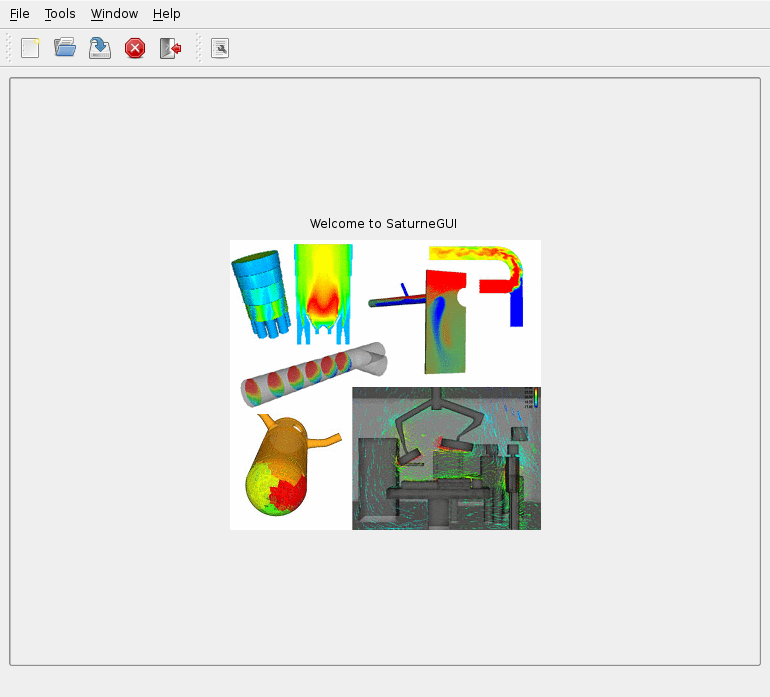
\includegraphics[width=13cm]{case1_V-1}
\caption{\CS (GUI) graphic window}
\label{fig1_e1}
\end{center}
\end{figure}


\clearpage
Go to the {\itshape File} menu and click on {\itshape New file} to open a new
calculation data file. The interface automatically updates the following information:
\begin{itemize}
        \item Study name
        \item Case name
        \item Directory of the case
        \item Associated sub-directories of the case
\end{itemize}

\begin{figure}[ht]
\begin{center}
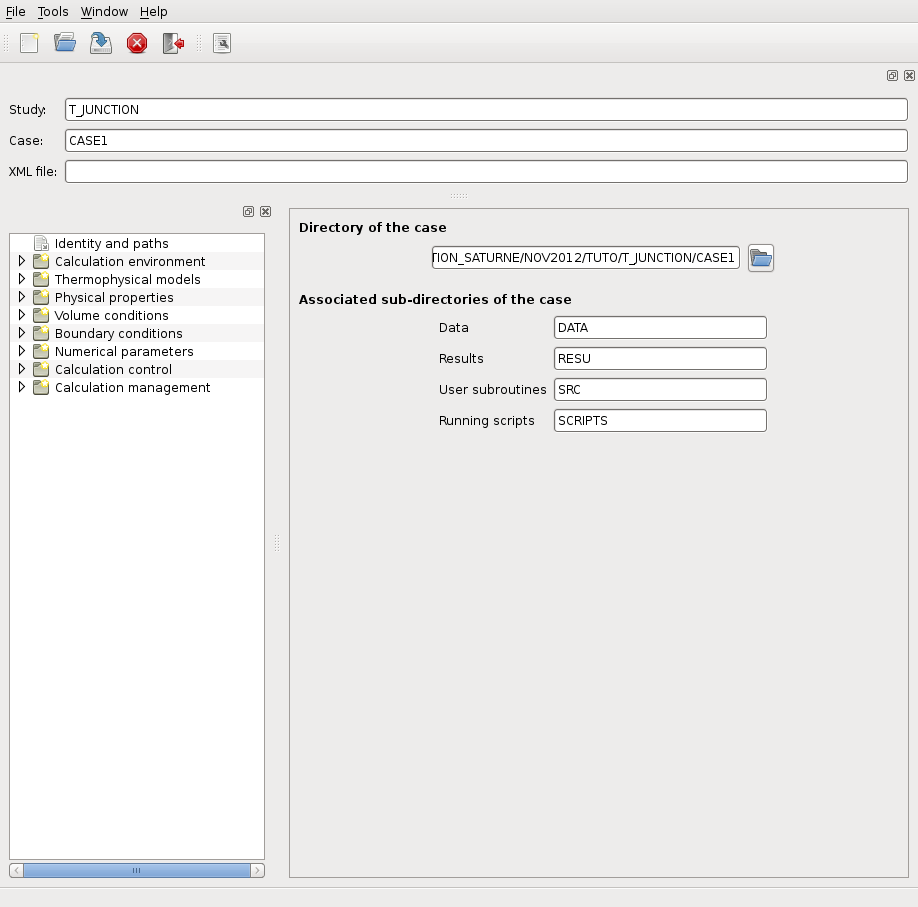
\includegraphics[width=12cm]{case1_V-2}
\caption{Identity and paths}
\label{fig2_e1}
\end{center}
\end{figure}


\clearpage
Save the case to give a name to the new \texttt{xml} file (such as \texttt{case1.xml})
by opening the {\itshape File} menu and clicking on {\itshape Save as...}.

A new window will appear, enter the name of the case in {\itshape File Name} then click on
{\itshape Save}.

Remember to save the case regularly throughout the preparation of the calculation.

\begin{figure}[ht]
\begin{center}
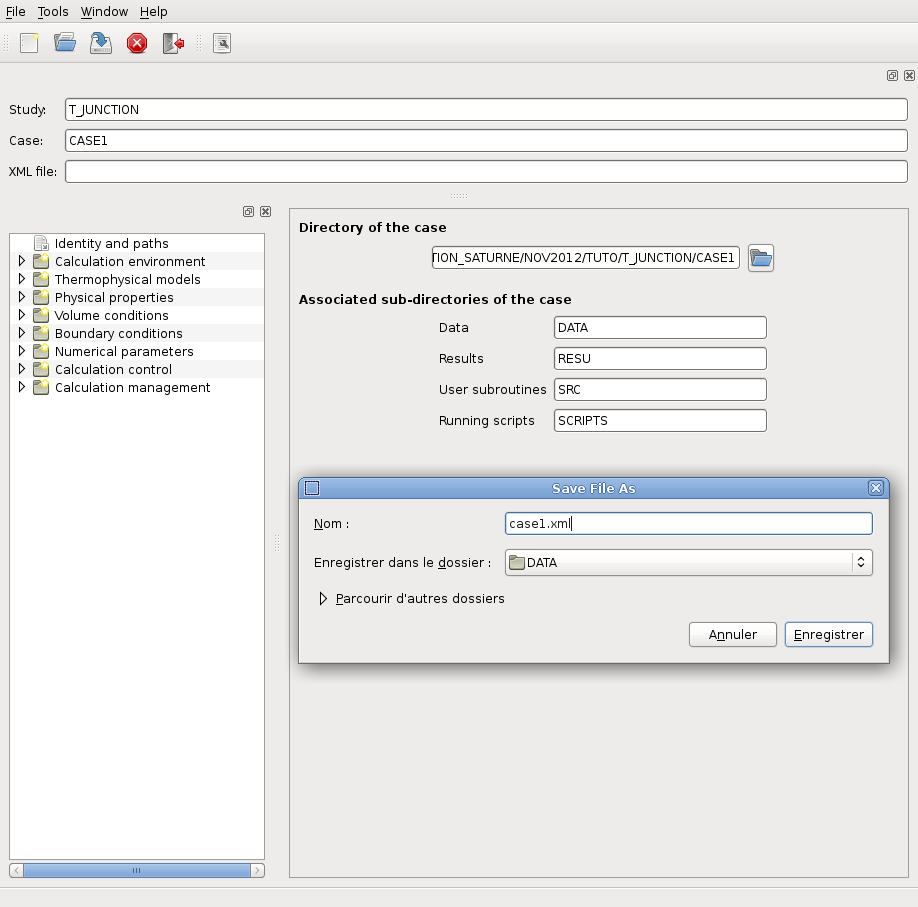
\includegraphics[width=10cm]{case1_V-3}
\caption{Saving the \texttt{xml} file}
\label{fig4_e1}
\end{center}
\end{figure}


\clearpage
The next step is to specify the mesh(es) to be used for the calculation.
Click on the {\itshape Mesh selection} item under the heading {\itshape Calculation environment}.
Click to {\bf ``+``} to add meshes.

The list of meshes in the folder {\itshape Meshes} appears in the window {\itshape List of meshes}.
In this case only the mesh \texttt{downcomer.des} is needed.

\begin{figure}[ht]
\begin{center}
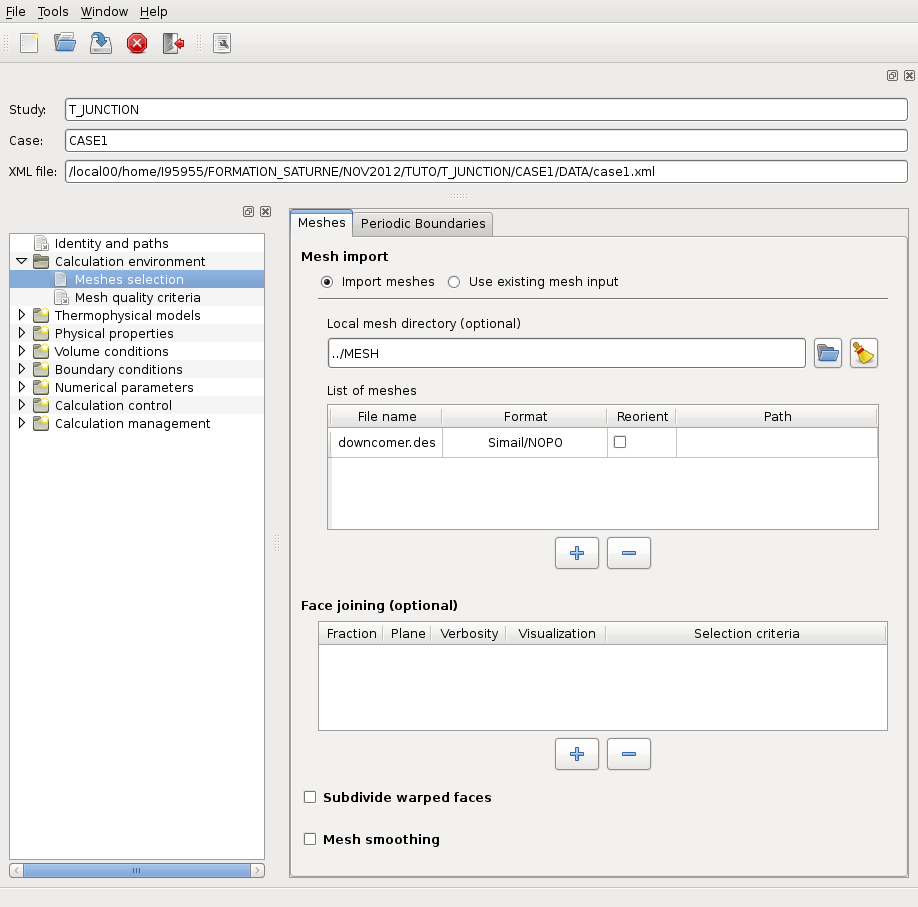
\includegraphics[width=12cm]{case1_V-4}
\caption{Meshes: list of meshes}
\label{fig5_e1}
\end{center}
\end{figure}

The {\itshape Periodic Boundaries} is not used in this case. Keep the default values.

\clearpage
The {\itshape Calculation features} item under the heading {\itshape Thermophysical
models} allows to define the type of flow to be simulated. In this case, a
steady flow will be chosen.

\begin{figure}[ht]
\begin{center}
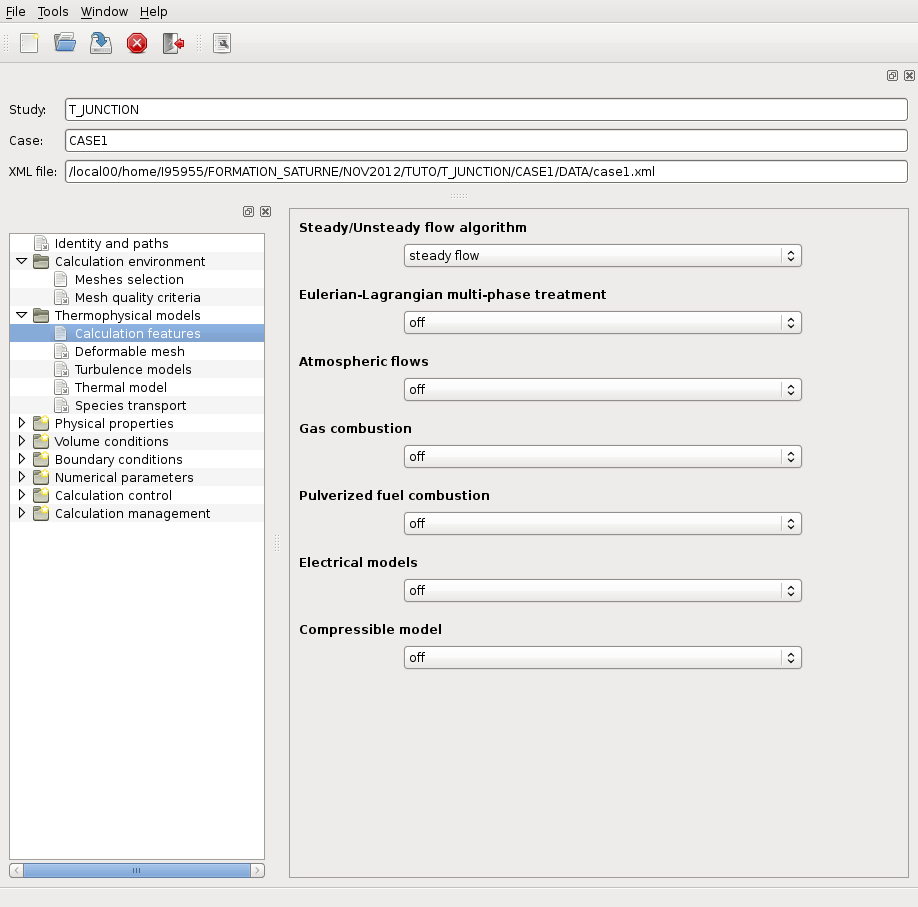
\includegraphics[width=12cm]{case1_V-5}
\caption{Flow type}
\label{fig7_e1}
\end{center}
\end{figure}


\clearpage
The turbulence model is selected in the following list:\\
\hspace*{1cm}$\bullet\ $laminar flow (no model)\\
\hspace*{1cm}$\bullet\ $mixing length\\
\hspace*{1cm}$\bullet\ $k-$\varepsilon$\\
\hspace*{1cm}$\bullet\ $k-$\varepsilon$ Linear Production\\
\hspace*{1cm}$\bullet\ $Rij-$\varepsilon$ LLR\\
\hspace*{1cm}$\bullet\ $Rij-$\varepsilon$ SSG\\
\hspace*{1cm}$\bullet\ $v2f ($\varphi$ model)\\
\hspace*{1cm}$\bullet\ $k-$\omega$ SST\\
\hspace*{1cm}$\bullet\ $Spalart-Allmaras\\
\hspace*{1cm}$\bullet\ $LES (Smagorinsky)\\
\hspace*{1cm}$\bullet\ $LES (classical dynamic model)\\
\hspace*{1cm}$\bullet\ $LES (WALE)

\begin{figure}[ht]
\begin{center}
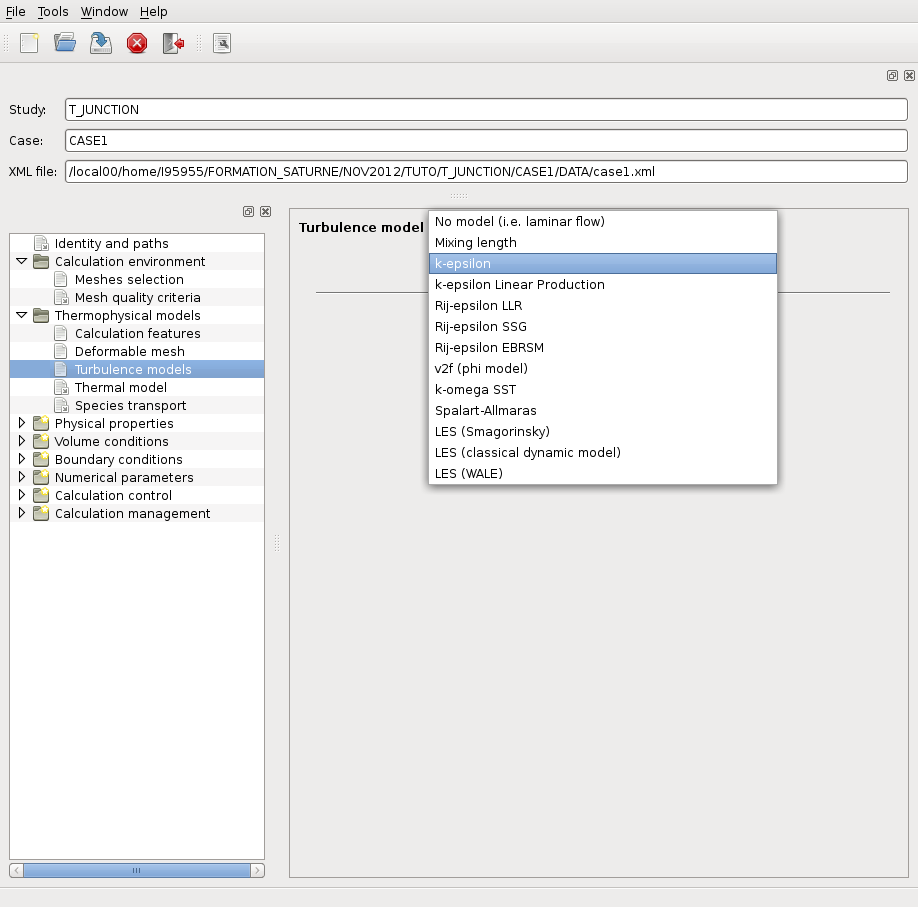
\includegraphics[width=12cm]{case1_V-6}
\caption{Turbulence model: list of models}
\label{fig9_e1}
\end{center}
\end{figure}


\clearpage
In this case, the k-$\varepsilon$ model is used.

\begin{figure}[ht]
\begin{center}
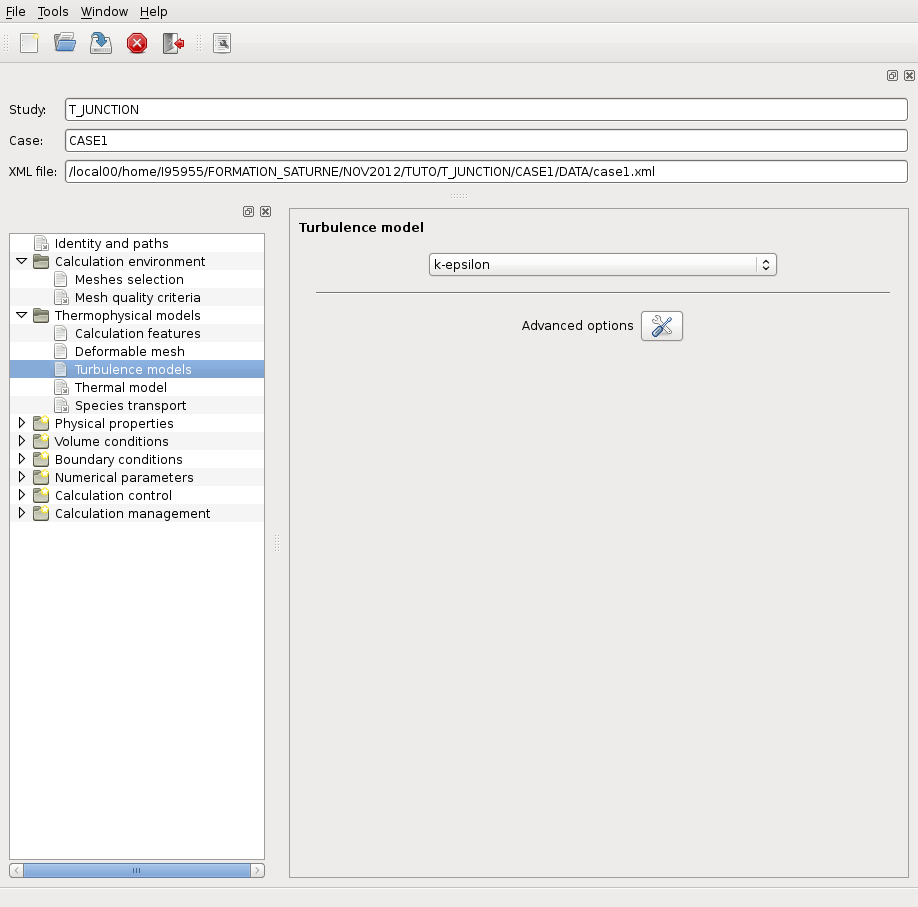
\includegraphics[width=9cm]{case1_V-7}
\caption{Turbulence model: choice of a model}
\label{fig10_e1}
\end{center}
\end{figure}


\clearpage
For this study the equation for temperature must be solved. Click on the
{\itshape Thermal model} item to
choose between:\\
\hspace*{1cm}$\bullet\ $No thermal scalar\\
\hspace*{1cm}$\bullet\ $Temperature (Celsius degrees)\\
\hspace*{1cm}$\bullet\ $Temperature (Kelvin)\\
\hspace*{1cm}$\bullet\ $Enthalpy

\begin{figure}[ht]
\begin{center}
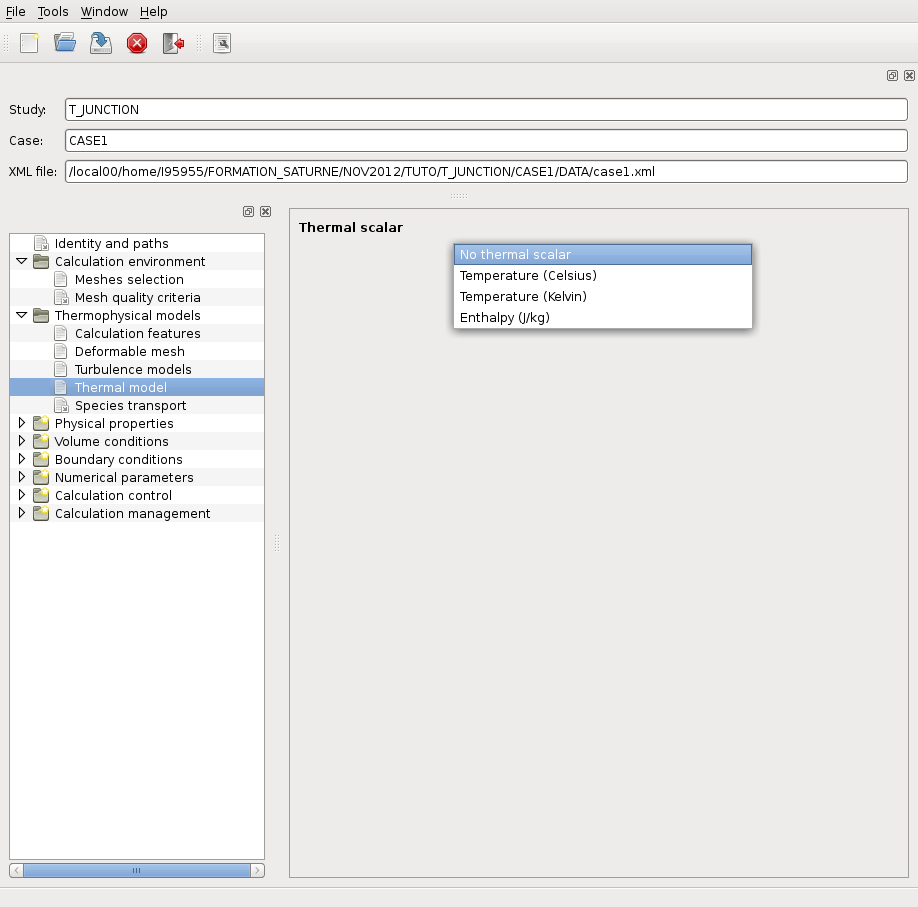
\includegraphics[width=12cm]{case1_V-8}
\caption{Thermal scalar conservation: list of models}
\label{fig11_e1}
\end{center}
\end{figure}


\clearpage
In the present case, select {\itshape Temperature (Celsius)}.
\begin{figure}[ht]
\begin{center}
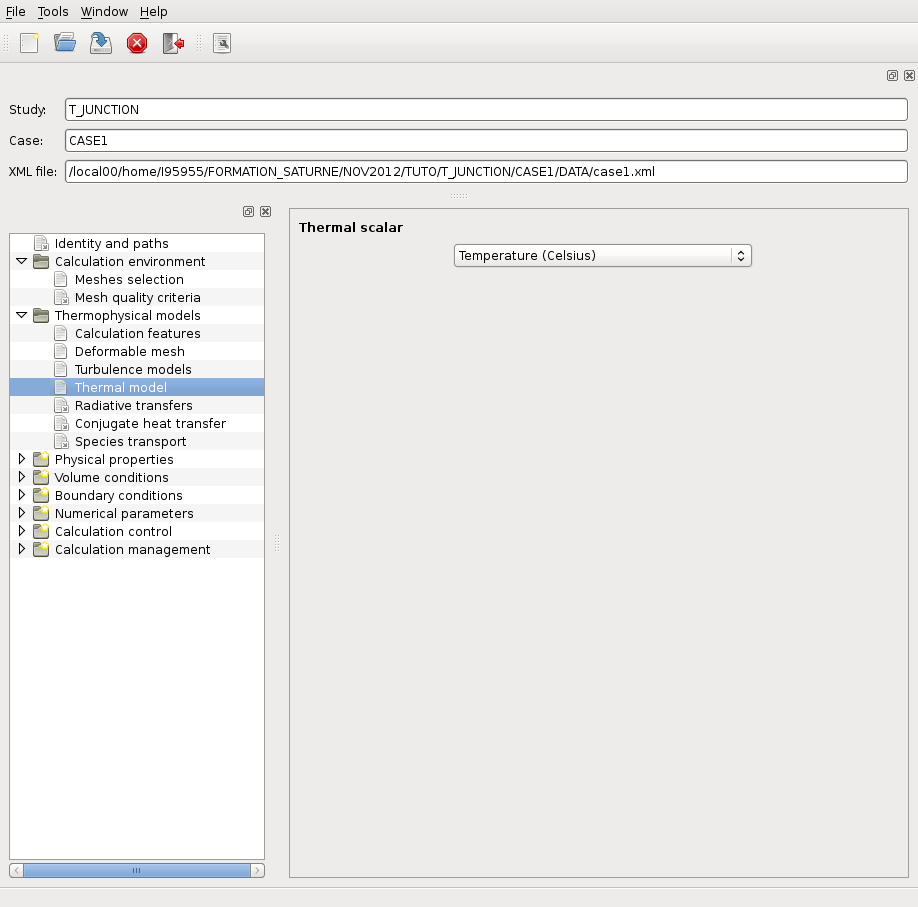
\includegraphics[width=9cm]{case1_V-9}
\caption{Thermal scalar conservation: choice of a model}
\label{fig12_e1}
\end{center}
\end{figure}

Once the thermal scalar selected, additional items appear.
There are no radiative transfers in our case, so this item can be ignored.

\clearpage
\textbf{Initialization:}

To initialize variables at the instant $t=0\ $($s$), go to the {\itshape Initialization} item
under the heading {\itshape Volume conditions}. Here the velocity, the thermal scalar and
the turbulence can be initialized.

In this case, the default values can be kept: zero velocity, an initial temperature
of {\bf 20}\degresC\  and a turbulence level based on a reference velocity of {\bf 1}
($m.s^{-1}$). Specific zones can be defined with different initializations.
In this case, only the default ``all cells'' is used.


\begin{figure}[ht]
\begin{center}
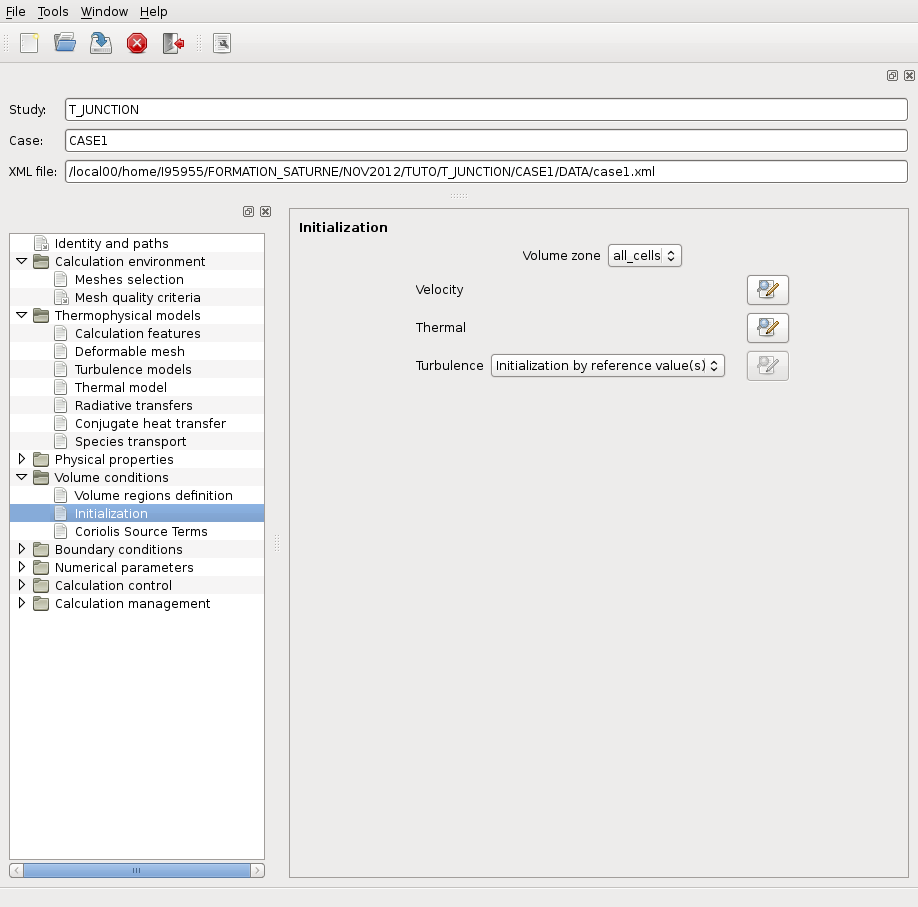
\includegraphics[width=12cm]{case1_V-10}
\caption{Initialization of the scalar, velocity and turbulence}
\label{fig15_e1}
\end{center}
\end{figure}
\begin{itemize}
\item Click on the icon near {\itshape ''Thermal''} in order to specify the initial value of
the thermal scalar. It can be a value or a user expression.

\clearpage
\begin{figure}[ht]
\begin{center}
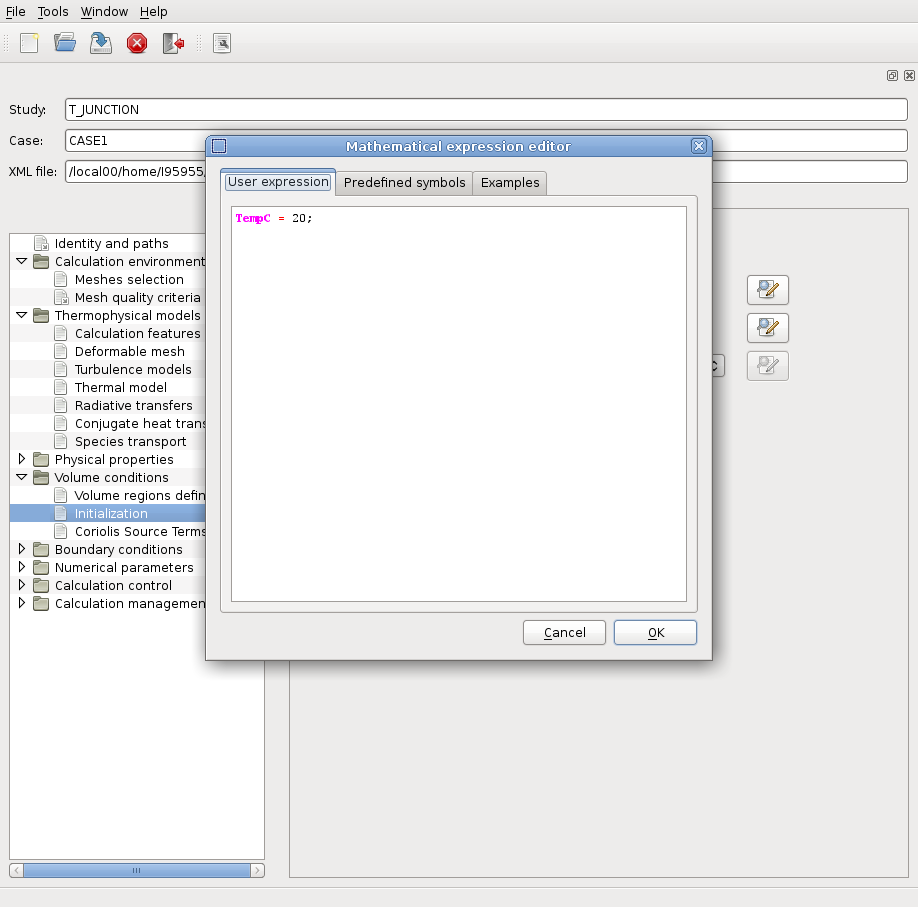
\includegraphics[width=12cm]{case1_V-11}
\caption{Initialization of the scalar}
\label{fig15_e1}
\end{center}
\end{figure}

\item To initialize the velocity, click also on the icon near  {\itshape ``Velocity''}.
\begin{figure}[ht]
\begin{center}
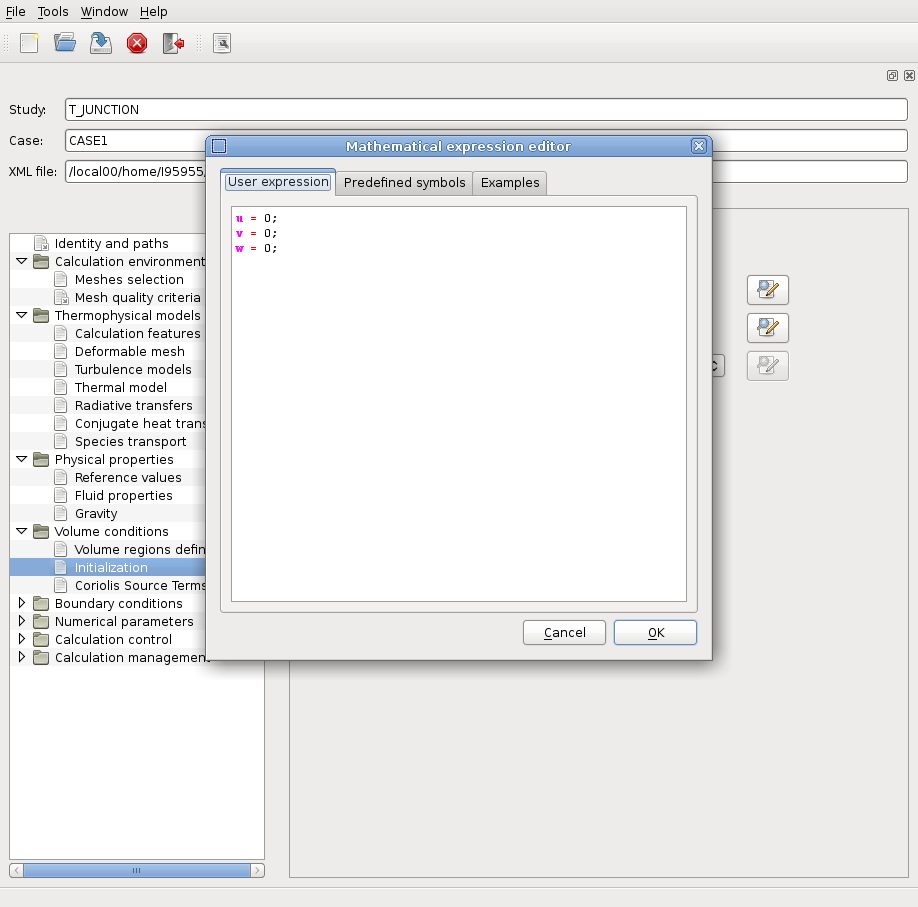
\includegraphics[width=12cm]{case1_V-12}
\caption{Initialization of the velocity}
\label{fig15_e1}
\end{center}
\end{figure}

\end{itemize}

\clearpage
Under the heading {\itshape Physical properties} in the main list, the {\itshape Reference values}
item allows to set the reference pressure, the reference velocity and the reference length.

Use the default value of {\bf 101 325} ($Pa$) for the pressure and {\bf 1} ($m/s$) for the velocity.

\begin{figure}[ht]
\begin{center}
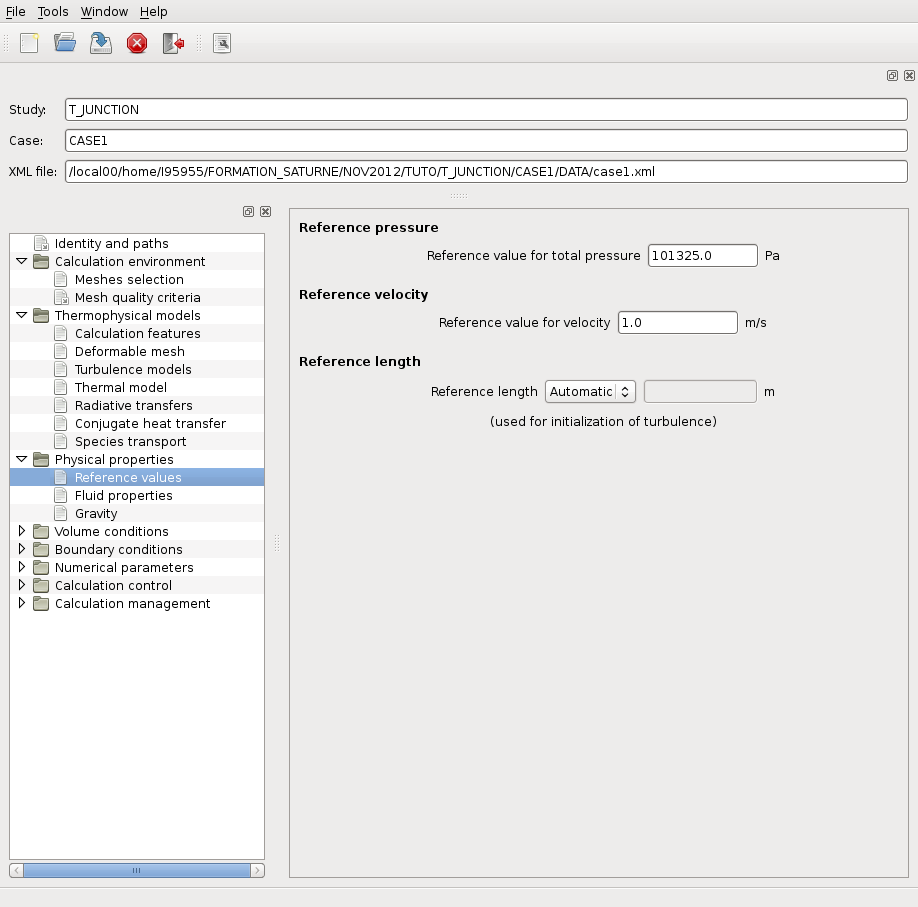
\includegraphics[width=12cm]{case1_V-13}
\caption{Physical properties: reference pressure}
\label{fig17_e1}
\end{center}
\end{figure}


\clearpage
Specify the fluid physical characteristics in the {\itshape Fluid
properties} item:
\begin{itemize}
        \item Density
        \item Viscosity
        \item Specific Heat
        \item Thermal Conductivity
\end{itemize}

In this case they are all constant.
\begin{itemize}
        \item $\rho~\qquad$ =$~  725.735\ kg.m^{-3}$
        \item $\mu~\qquad$  =$~  0.895\times 10^{-4}\ kg.m^{-1}.s^{-1}$
        \item $C_p~~\quad$ =$~ 5\,483\ J.kg^{-1}.\mbox{\degresC}^{-1}$
        \item $(\lambda/C_p)$ =$~ 0.02495\ W.m^{-1}.K^{-1}$
\end{itemize}

\begin{figure}[ht]
\begin{center}
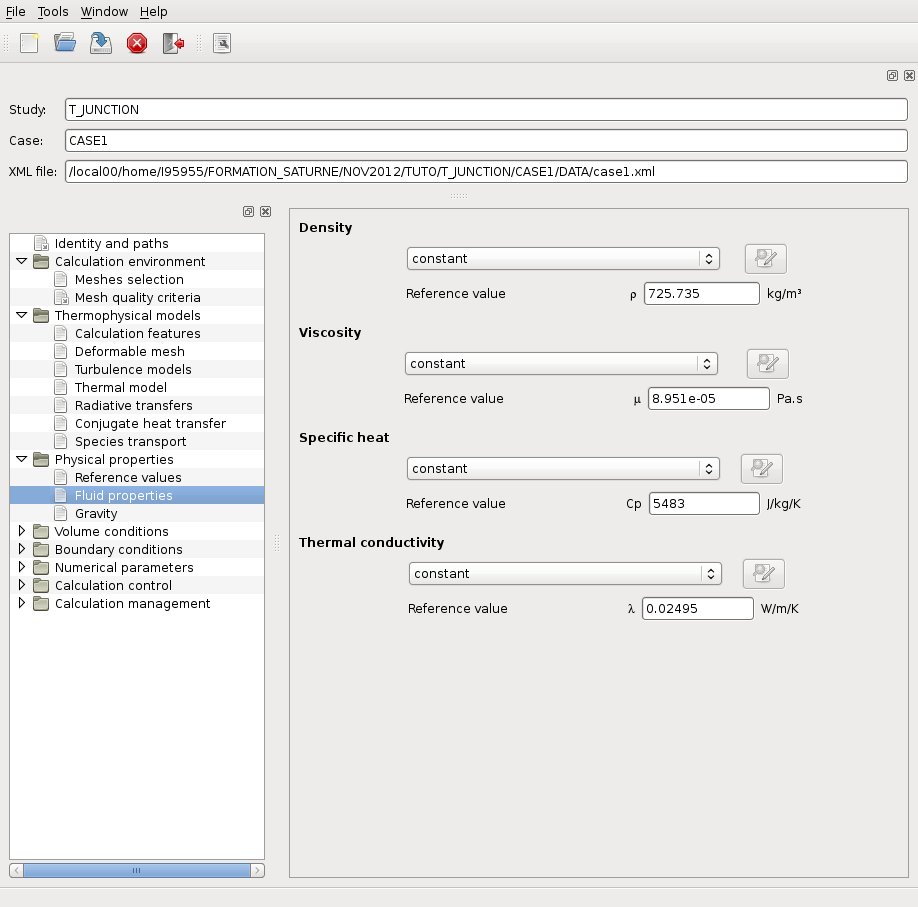
\includegraphics[width=12cm]{case1_V-14}
\caption{Physical properties: fluid properties}
\label{fig18_e1}
\end{center}
\end{figure}


\clearpage
Set the three components of gravity in the
{\itshape Gravity} item. In this case, since the gravity doesn't have any
influence on the flow, gravity can be set to {\bf 0}.

As for the pressure interpolation, the interpolation method keeps the standard
default value.

\begin{figure}[ht]
\begin{center}
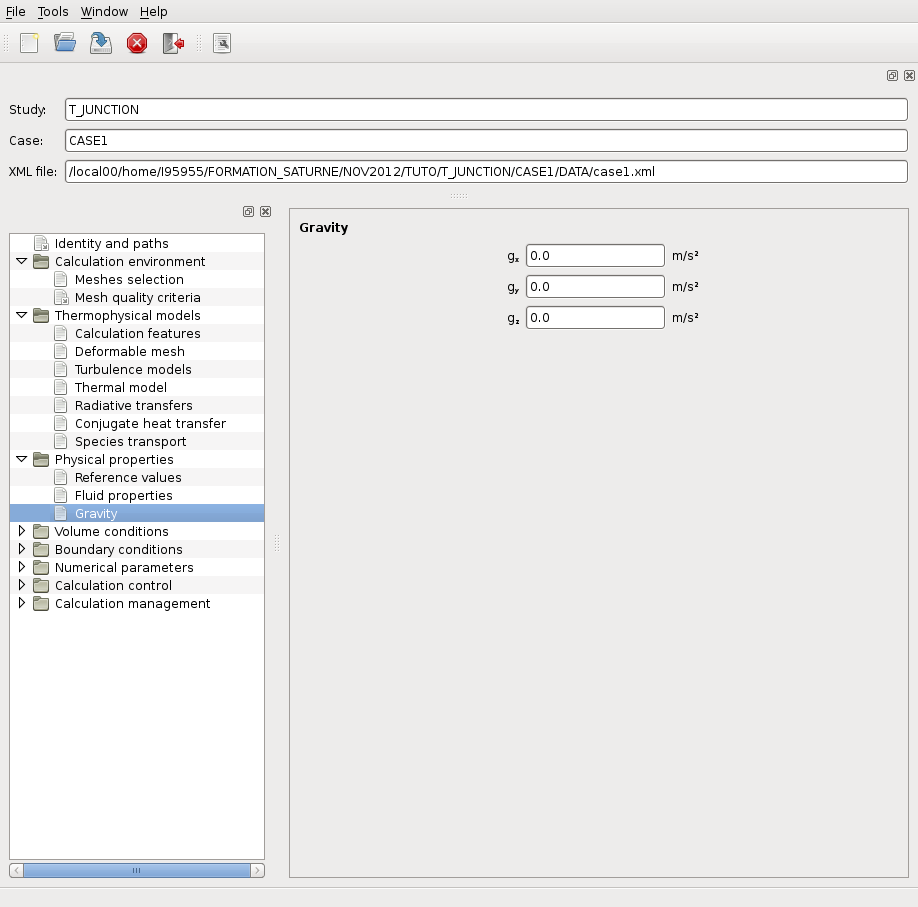
\includegraphics[width=12cm]{case1_V-15}
\caption{Physical properties: gravity and hydrostatic pressure}
\label{fig19_e1}
\end{center}
\end{figure}


\clearpage
Boundary conditions now need to be defined. Go to the {\itshape Define
boundary regions} item under the heading {\itshape Boundary conditions}.
The following window opens (fig \ref{fig20_e1}).

\begin{figure}[ht]
\begin{center}
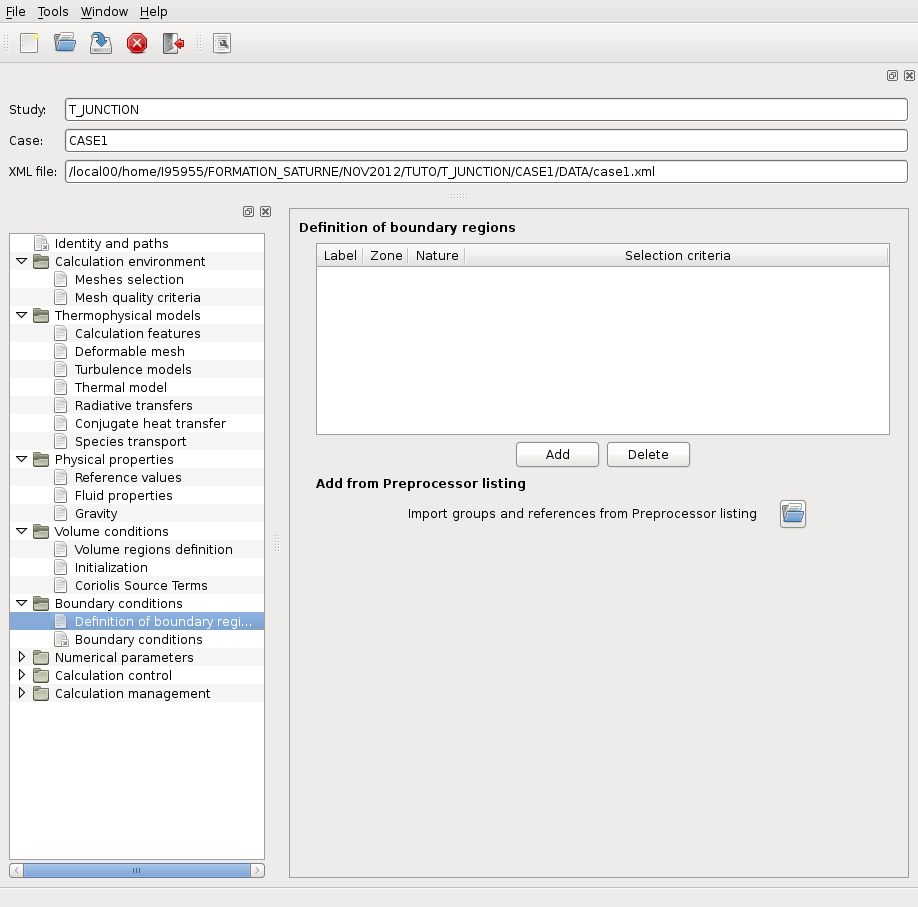
\includegraphics[width=12cm]{case1_V-16}
\caption{Creation of a boundary region}
\label{fig20_e1}
\end{center}
\end{figure}


\clearpage
Each boundary must be defined. Click on {\itshape Add} to edit a new boundary.
The boundary faces will be grouped in
user-defined zones, based on their color or on geometrical conditions. For each
zone, a reference number, a label, a nature and a selection criteria must be
assigned.
The different natures that can be assigned are:\\
\fbox{\begin{minipage}{\textwidth}\texttt{    \\
- wall                                        \\
- inlet                                       \\
- symmetry                                    \\
- outlet
}\end{minipage} }

The {\itshape Label} can be any character string. It is used to identify the
zone more easily. It usually corresponds to the nature of the zone.

The {\itshape Zone} number can be any integer. It will be used by the code to
identify the zone. No specific order or continuity in the numbering is needed.

The {\itshape Selection criteria} is used to define the faces that belong to the
zone. It can be a color number, a group reference, geometrical conditions, on a
combination of them, related by \texttt{``or''} or \texttt{``and''} keywords.

\begin{figure}[ht]
\begin{center}
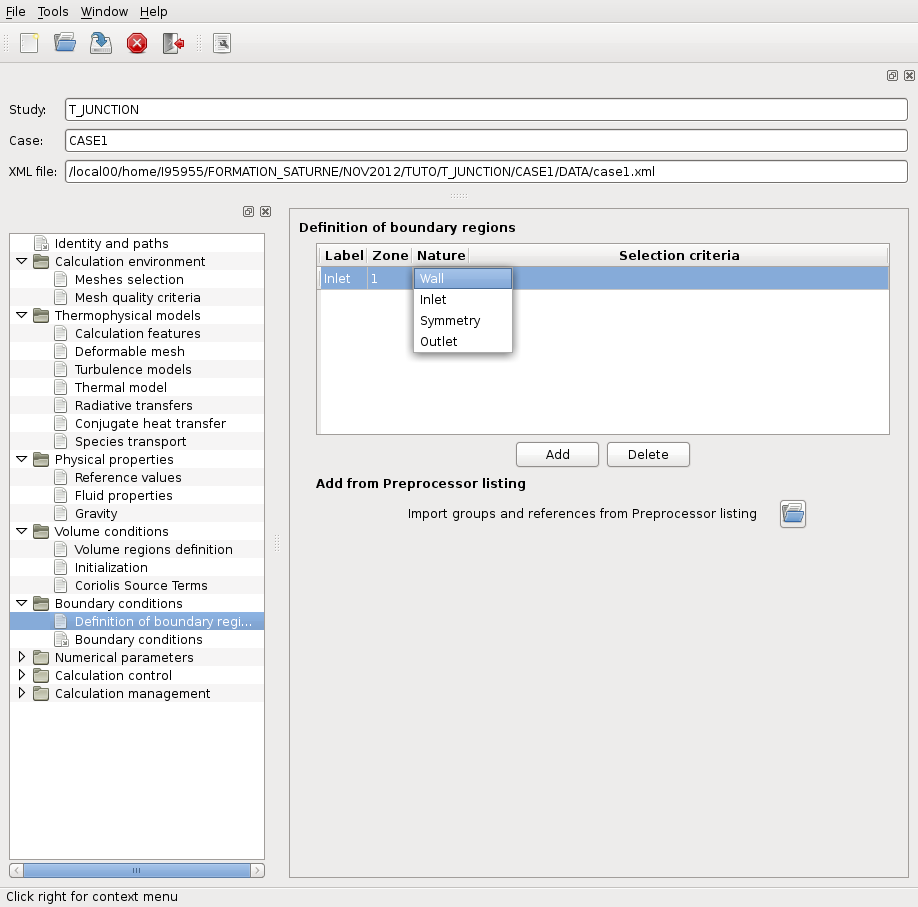
\includegraphics[width=8cm]{case1_V-17}
\caption{Creation of a boundary region}
\label{fig21_e1}
\end{center}
\end{figure}


\clearpage
The specification of the inlet condition is detailled in the following
pages. The settings will be as follows:\\
\fbox{\begin{minipage}{\textwidth}\texttt{    \\
 Label: inlet, \\
 Zone: 1, \\
 Nature: inlet,\\
 Selection criteria: 1
}\end{minipage} }

Type all the information in the fields, the result diplays as figure \ref{fig20_e1}

\begin{figure}[ht]
\begin{center}
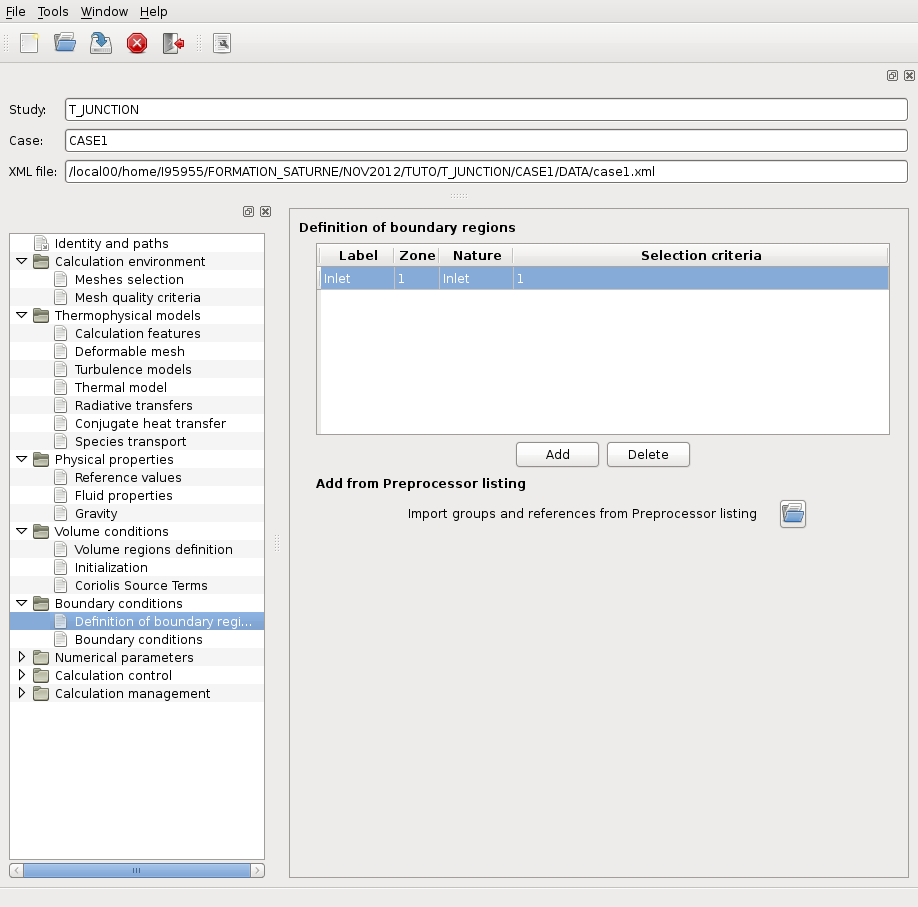
\includegraphics[width=8cm]{case1_V-18}
\caption{Creation of a boundary region}
\label{fig20_e1}
\end{center}
\end{figure}

Remember to save the \texttt{xml} file regularly!


\clearpage
Do the same thing for the other boundaries.

In our case, colors 8 and 9 are symmetry boundaries. One option can be to define
a separate zone for each color, as follows:
\begin{center}
\begin{tabular}{|l|c||c|}
\hline
Label & symmetry\_1 & symmetry\_2 \\
\hline
\hline
Zone & 3 & 4 \\
\hline
Nature & symmetry & symmetry \\
\hline
Localization & 8  & 9 \\
\hline
\end{tabular}
\end{center}

But it is usually faster to regroup the different colors in one single zone, as
shown on figure \ref{fig24_e1}. In our case, the localization for this zone is
the string \texttt{``8 or 9''}.

\begin{figure}[ht]
\begin{center}
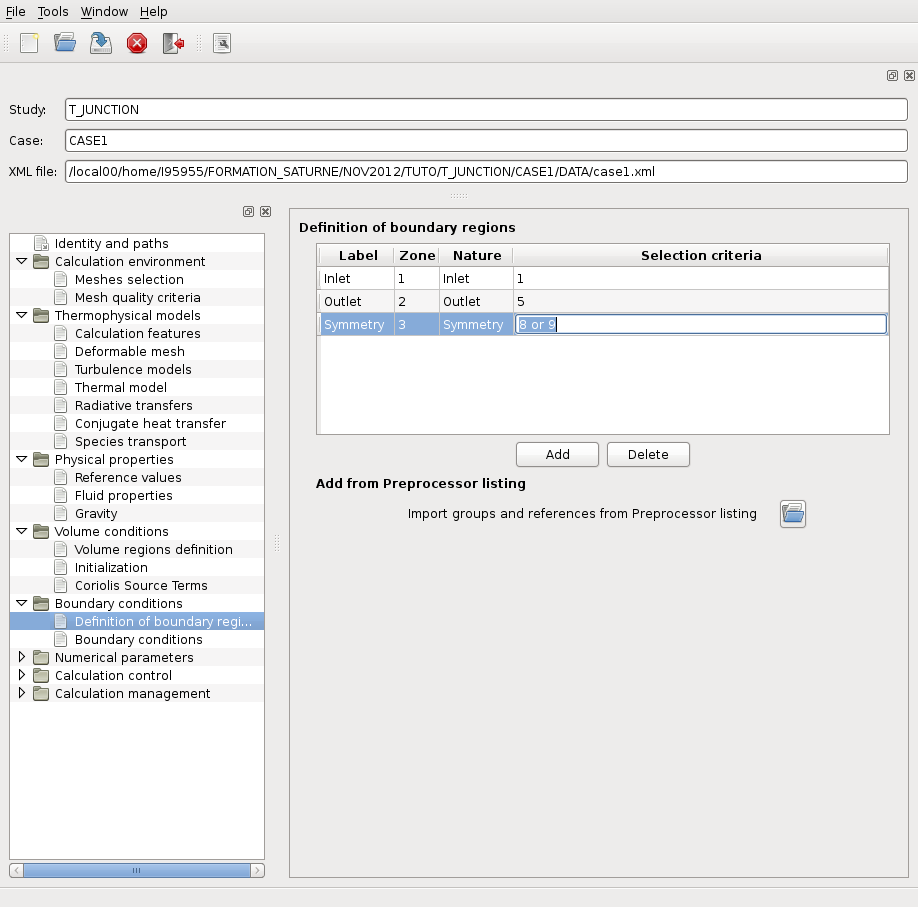
\includegraphics[width=8cm]{case1_V-19}
\caption{Creation of boundary regions: symmetry region}
\label{fig24_e1}
\end{center}
\end{figure}


\clearpage
The same treatment must be done for the wall conditions. All colors 2, 3, 4, 6
and 7 can be grouped in a single boundary zone.

After defining all the boundary zones, the Interface window will look as in
figure \ref{fig25_e1}.

\begin{figure}[ht]
\begin{center}
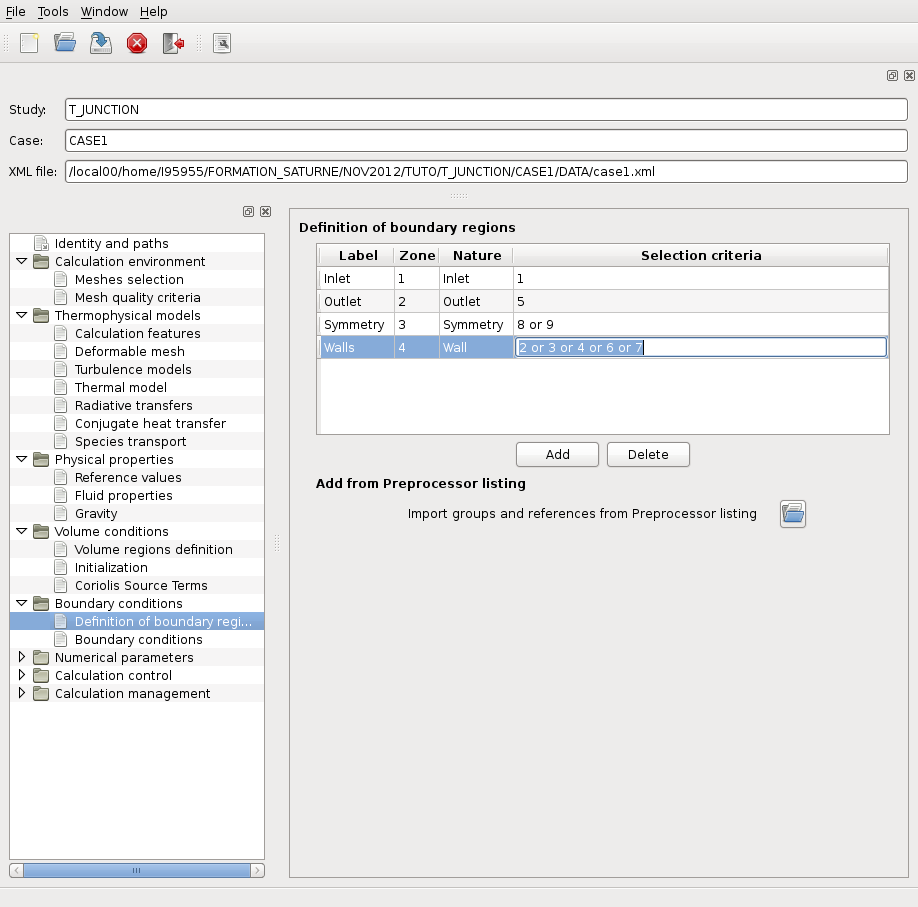
\includegraphics[width=8cm]{case1_V-20}
\caption{Creation of boundary regions}
\label{fig25_e1}
\end{center}
\end{figure}


\clearpage
Now that the boundary zones are defined, the boundary conditions assigned to
them will be specified. Click on the {\itshape Boundary conditions} item to
set the inlet boundary conditions for velocity, turbulence and themal scalar.

As shown on figure \ref{fig26_e1}, outlet and wall boundary zones also
appear in the window.

\begin{figure}[ht]
\begin{center}
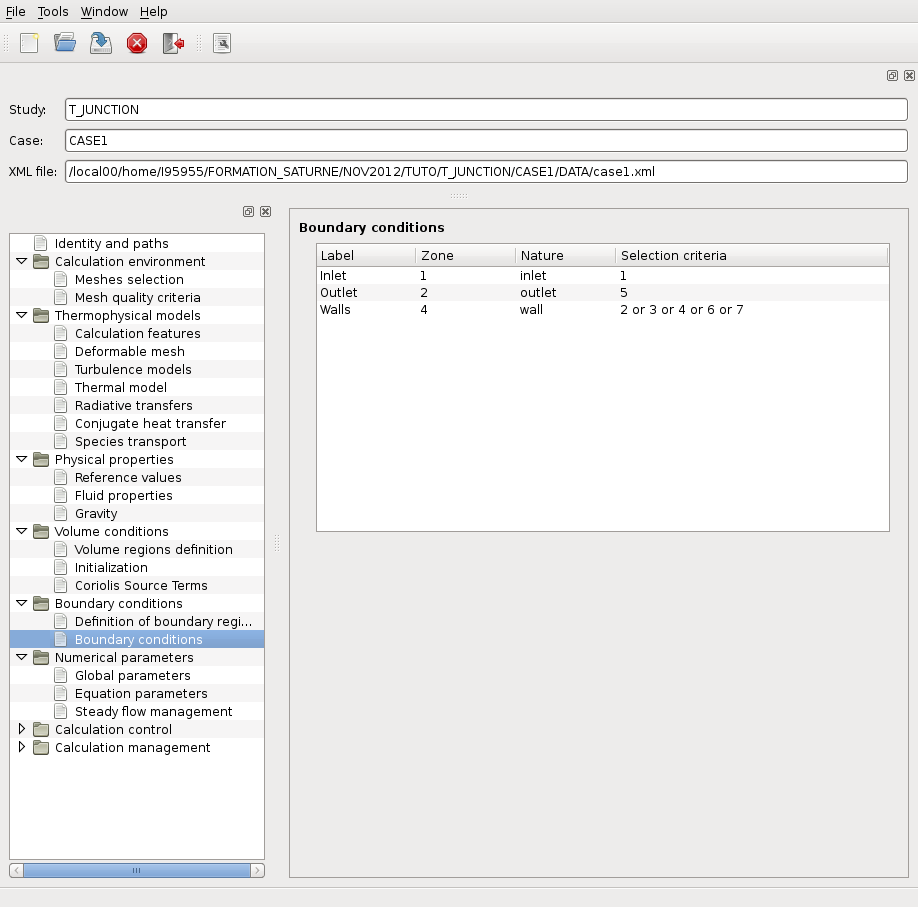
\includegraphics[width=12cm]{case1_V-21}
\caption{Dynamic variables boundary conditions}
\label{fig26_e1}
\end{center}
\end{figure}

\clearpage
Click on the label {\itshape inlet}. In the section {\itshape Velocity},
select {\itshape norm}, then in the sub-section {\itshape Direction} choose
{\itshape specified coordinates} and enter the normal vector components of
the inlet velocity.

For the turbulence, choose the inlet condition based on a hydraulic diameter
and specify it as below:\\
\fbox{\begin{minipage}{\textwidth}\texttt{    \\
 x = 1.0 (m) ; y = 0.0 (m) ; z = 0.0 (m) \\
 hydraulic diameter = 0.5 (m)
}\end{minipage} }

\begin{figure}[ht]
\begin{center}
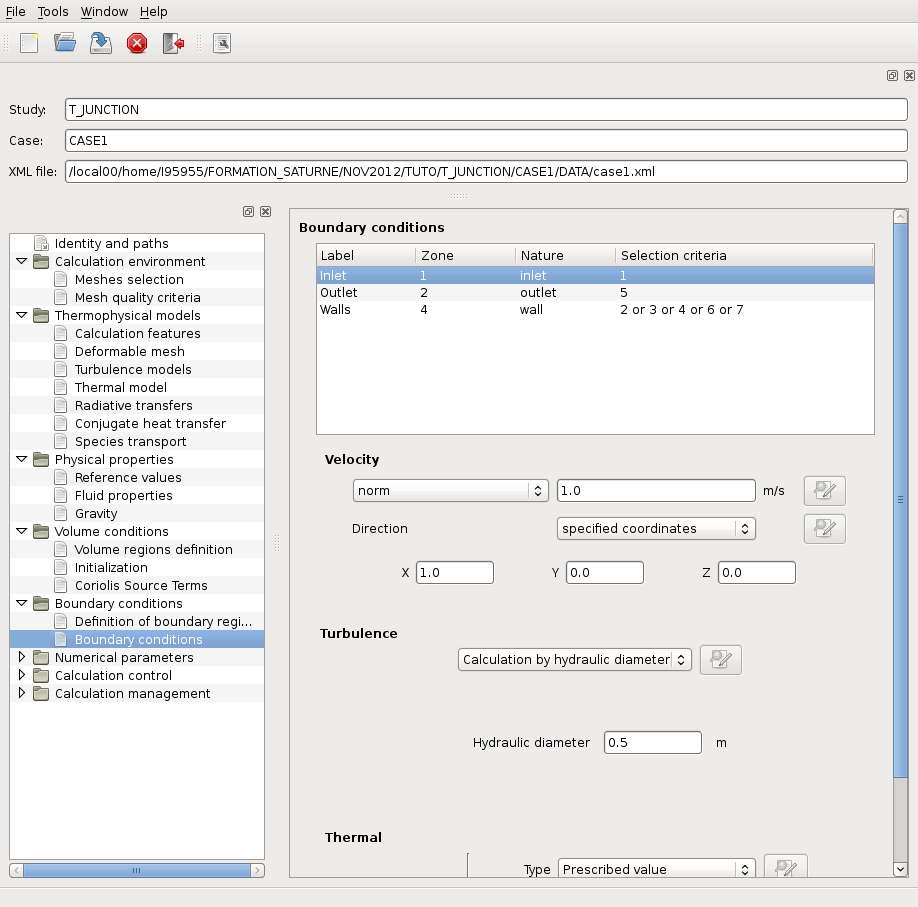
\includegraphics[width=9cm]{case1_V-22}
\caption{Dynamic variables boundary conditions: inlet}
\label{fig27_e1}
\end{center}
\end{figure}

Click on {\itshape inlet} to choose the temperature inlet
value. Here this value is {\bf 300}\degresC.
\begin{figure}[ht]
\begin{center}
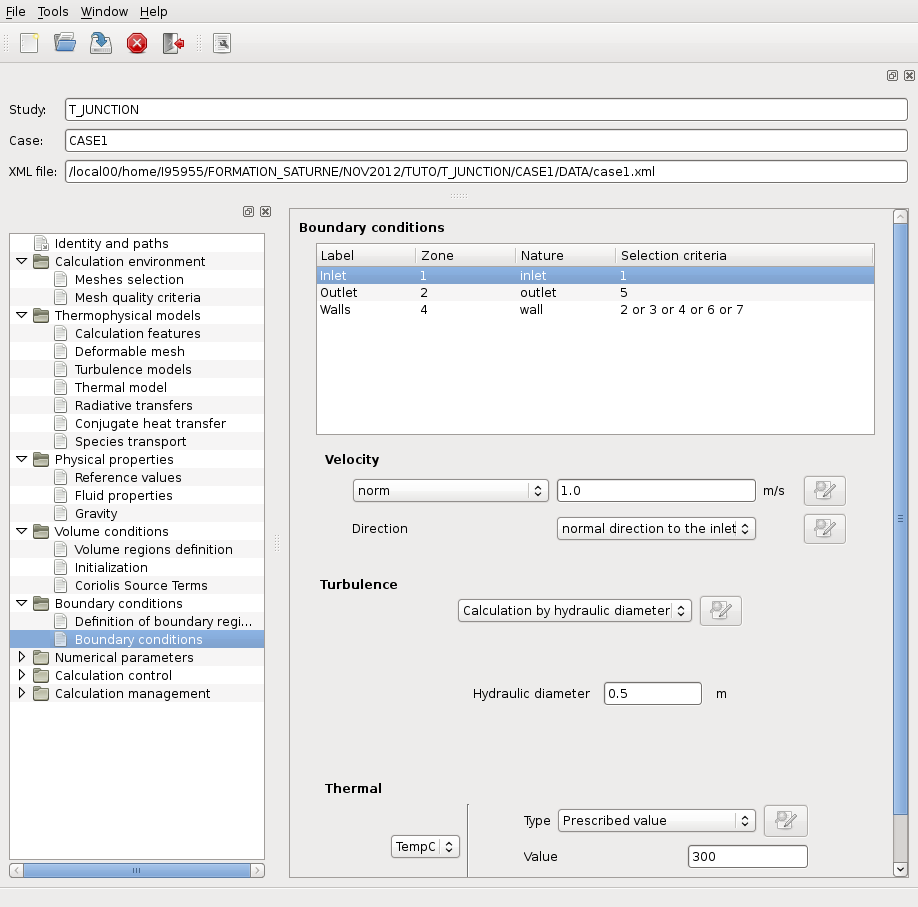
\includegraphics[width=12cm]{case1_V-23}
\caption{Dynamic variables boundary conditions: inlet}
\label{fig26_e1}
\end{center}
\end{figure}

\clearpage
As for the wall boundary zone, the specifications the user might have to
give is when the wall is sliding, and if the wall is \texttt{"smooth"}
or \texttt{"rough"}. In this case, the walls are fixed so the option is
not selected, and the wall is considered as \texttt{"smooth"}.

Note that if one of the walls had been sliding, it would have been necessary to
isolate the corresponding boundary faces in a specific boundary region.

\begin{figure}[ht]
\begin{center}
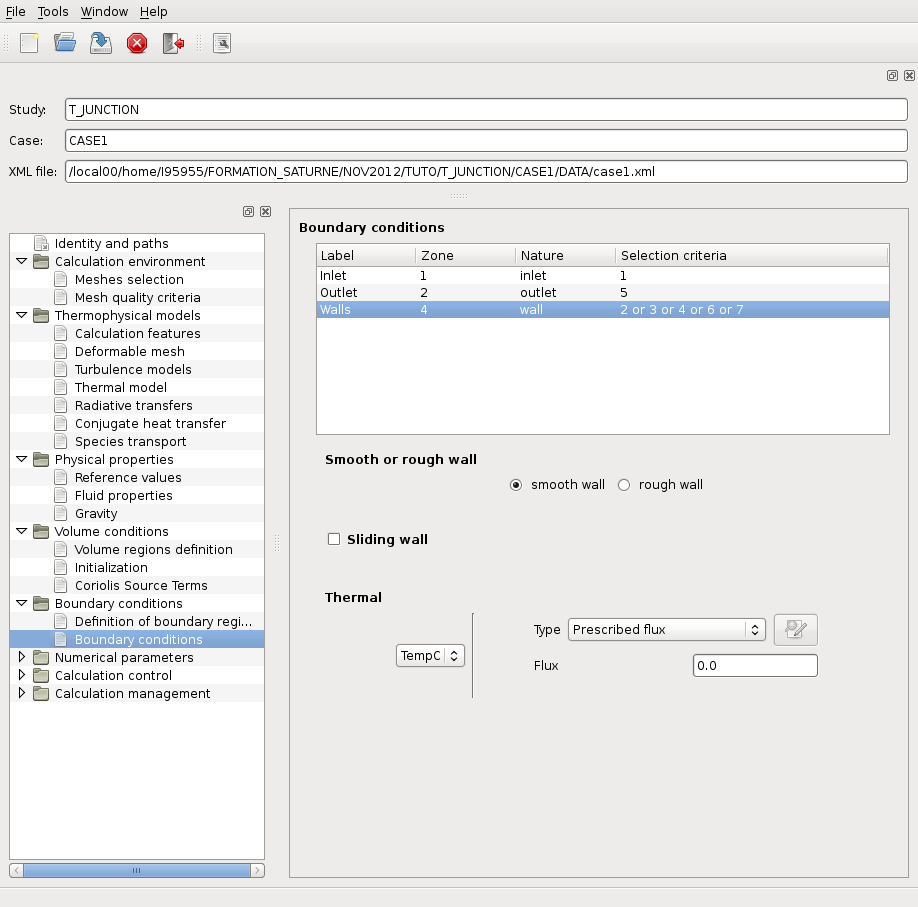
\includegraphics[width=9cm]{case1_V-24}
\caption{Dynamic variables boundary: walls}
\label{fig28_e1}
\end{center}
\end{figure}


\clearpage
The boundary conditions
on the temperature are only applied on inlets, outlets and walls.

For the walls, three conditions are available:\\
\fbox{\begin{minipage}{\textwidth}\texttt{    \\
- Prescribed value                            \\
- Prescribed flux                             \\
- Exchange Coefficient
}\end{minipage} }

For the outlet, only {\itshape Prescribed value} and {\itshape Prescribed flux}
are available, but they are taken into account only when the flow re-enters
from the outlet. Otherwise, homogeneous {\itshape Prescribed flux} is
considered by \CS.

For the inlets, only {\itshape Prescribed value} is available.

In this case all walls are adiabatic. So the boundary condition for the
temperature will be a {\itshape Prescribed flux} set to {\bf 0}.
\begin{figure}[ht]
\begin{center}
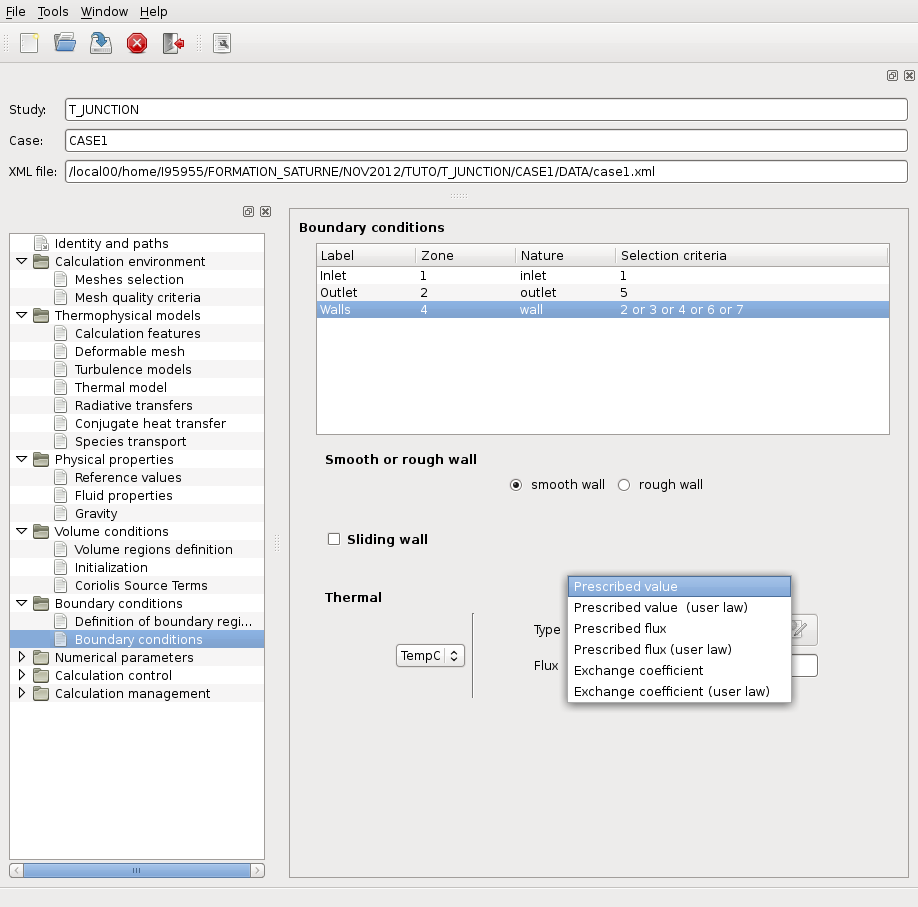
\includegraphics[width=10cm]{case1_V-25}
\caption{Scalars boundaries: walls}
\label{fig30_e1}
\end{center}
\end{figure}


\clearpage
The Global parameters need then to be specified, under the header {\itshape
Numerical parameters}. In this case, the SIMPLE algorithm must be chosen
\begin{figure}[ht]
\begin{center}
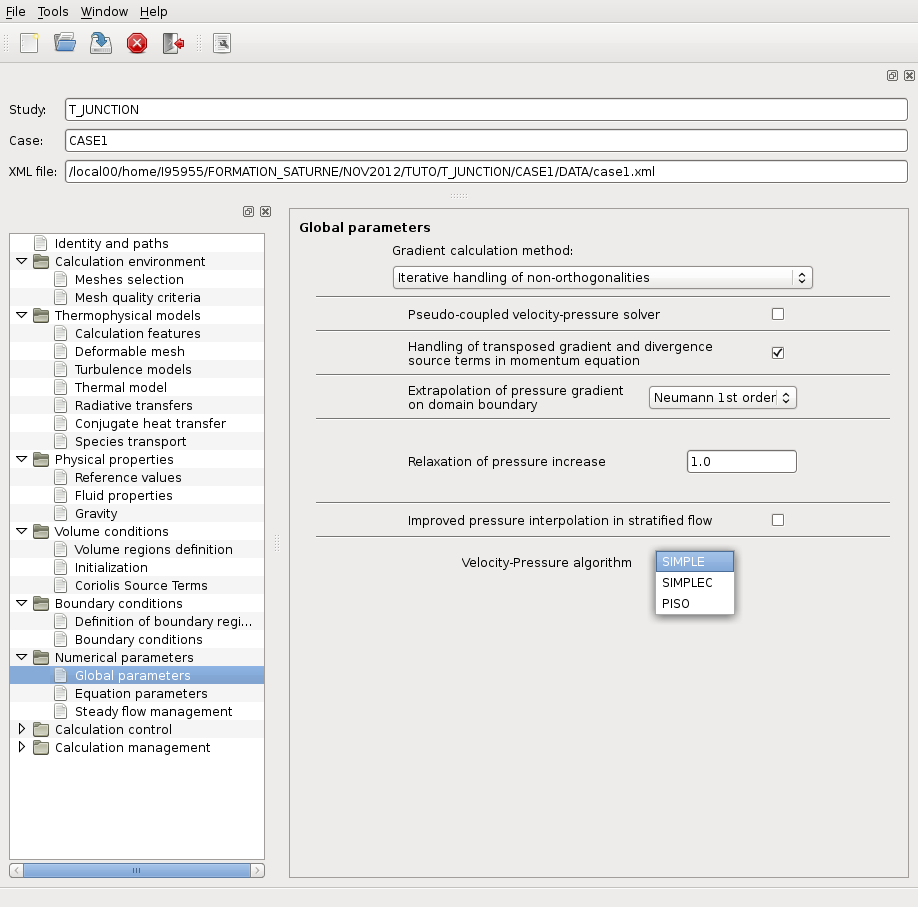
\includegraphics[width=12cm]{case1_V-26}
\caption{Steady flow management}
\label{fig32_e1}
\end{center}
\end{figure}


\clearpage
After selecting the {\itshape Equation parameters} item, the tab {\itshape Scheme}
allows to change different more advanced numerical parameters.

In this case none of them should be changed from their default value.

\begin{figure}[!h]
\begin{center}
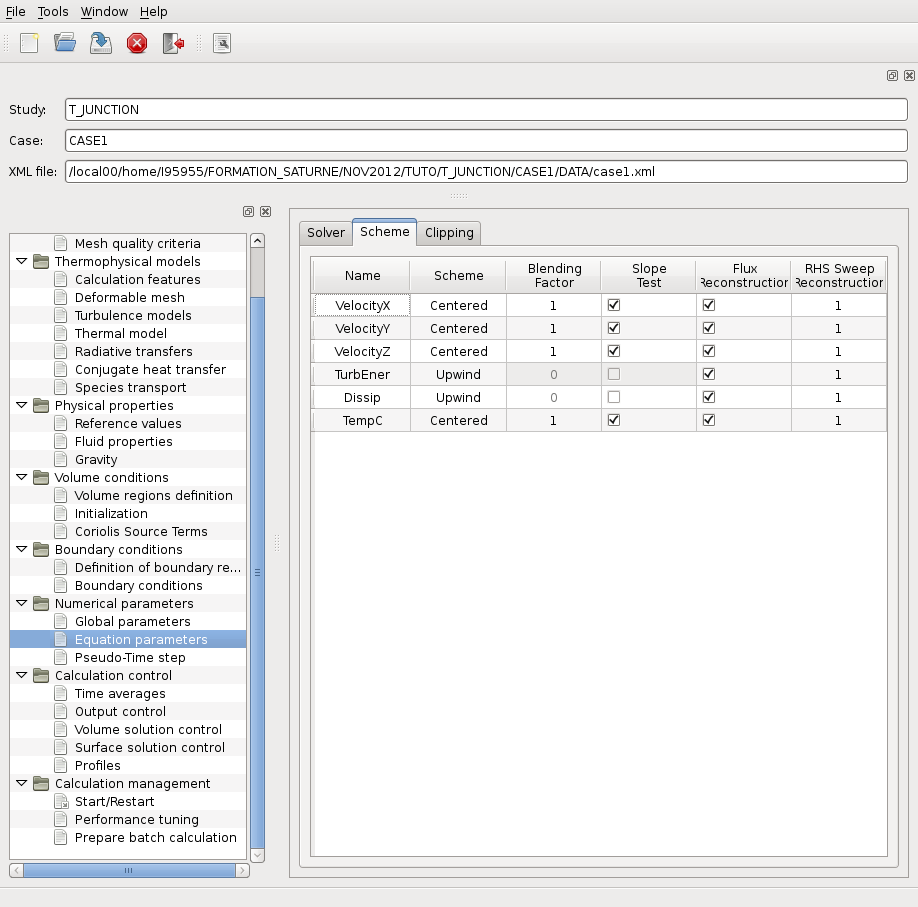
\includegraphics[width=11cm]{case1_V-27}
\caption{Numerical parameters}
\label{fig3738_e1}
\end{center}
\end{figure}
\clearpage
The tab {\itshape Clipping} in the {\itshape Equation parameters} item permits
to vanish the too small or too big value.
\begin{figure}[!h]
\begin{center}
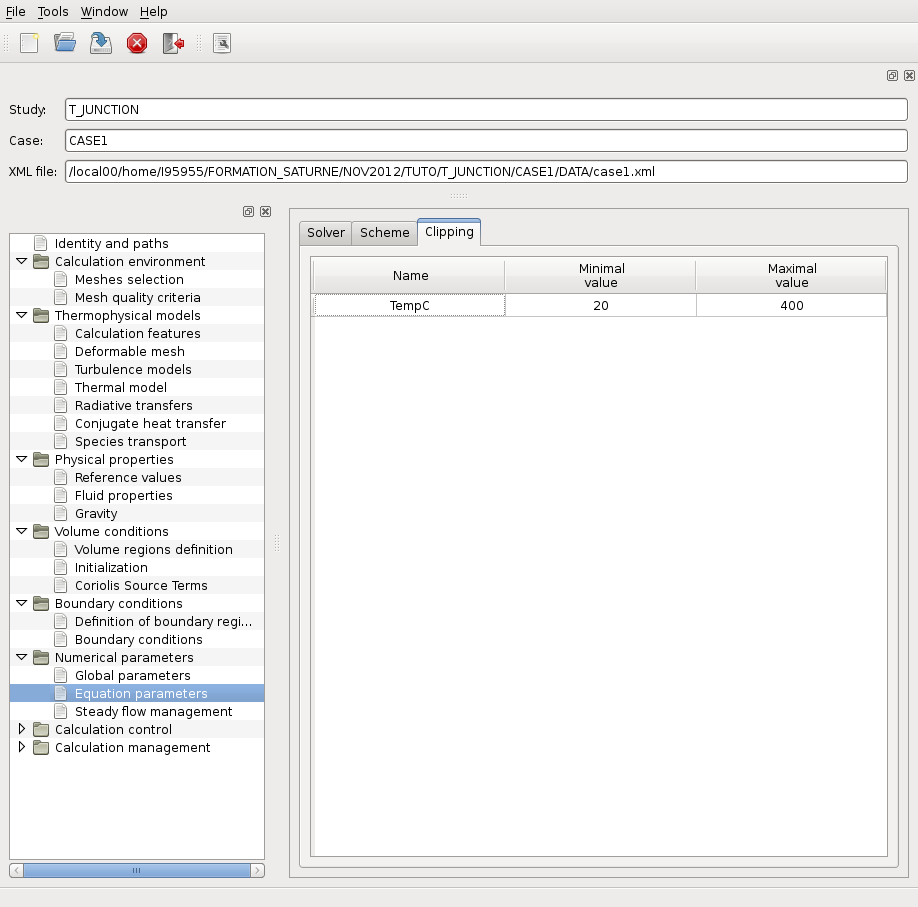
\includegraphics[width=11cm]{case1_V-28}
\caption{Clipping}
\label{fig3738_e1}
\end{center}
\end{figure}
\clearpage
Go to the {\itshape Steady flow management} item to specify the number of
iterations, {\bf 300} in this case. The relaxation coefficient is equal to {\bf 0.9} and
the {\itshape Zero iteration option} will not be activated.

\begin{figure}[ht]
\begin{center}
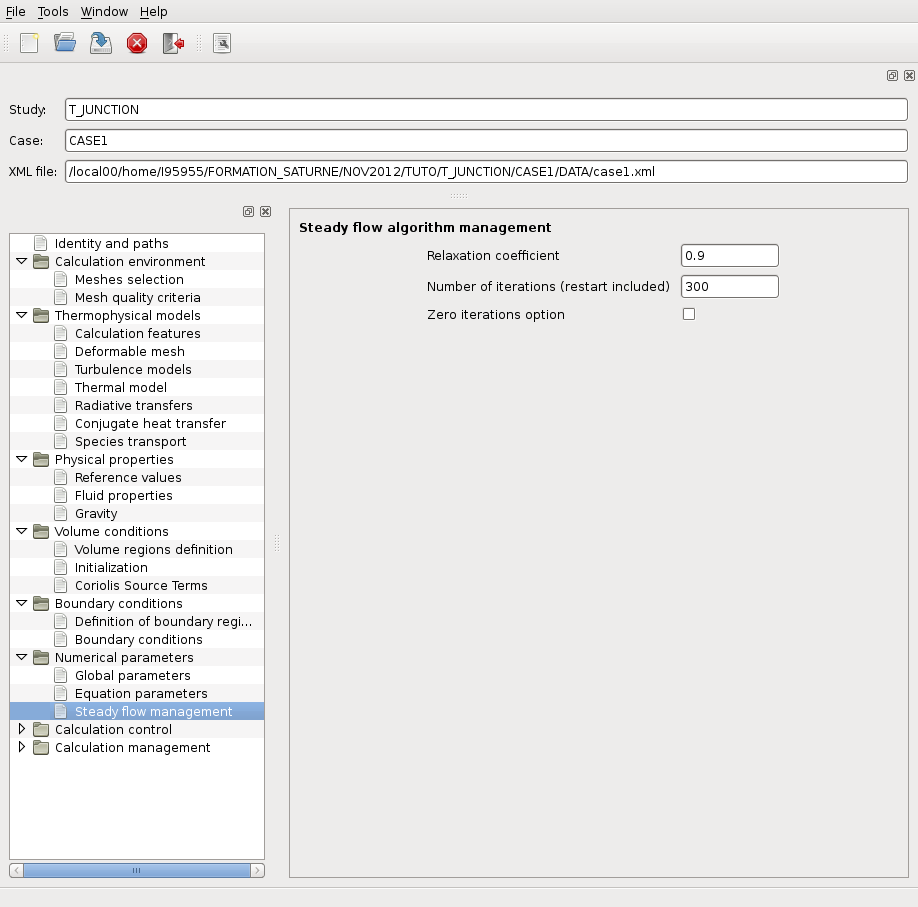
\includegraphics[width=12cm]{case1_V-29}
\caption{Steady flow management}
\label{fig32_e1}
\end{center}
\end{figure}
\clearpage
Under the heading {\itshape Calculation control}, click on the {\itshape Output control}
item to change the frequency for the printing of information in the output listing.

The options are:\\
\fbox{\begin{minipage}{\textwidth}\texttt{    \\
- No output\\
- Output listing at each time step\\
- Output at each 'n' time step (the value of 'n' must then be specified)
}\end{minipage} }
Here and in most cases, the second option should be chosen.

\begin{figure}[ht]
\begin{center}
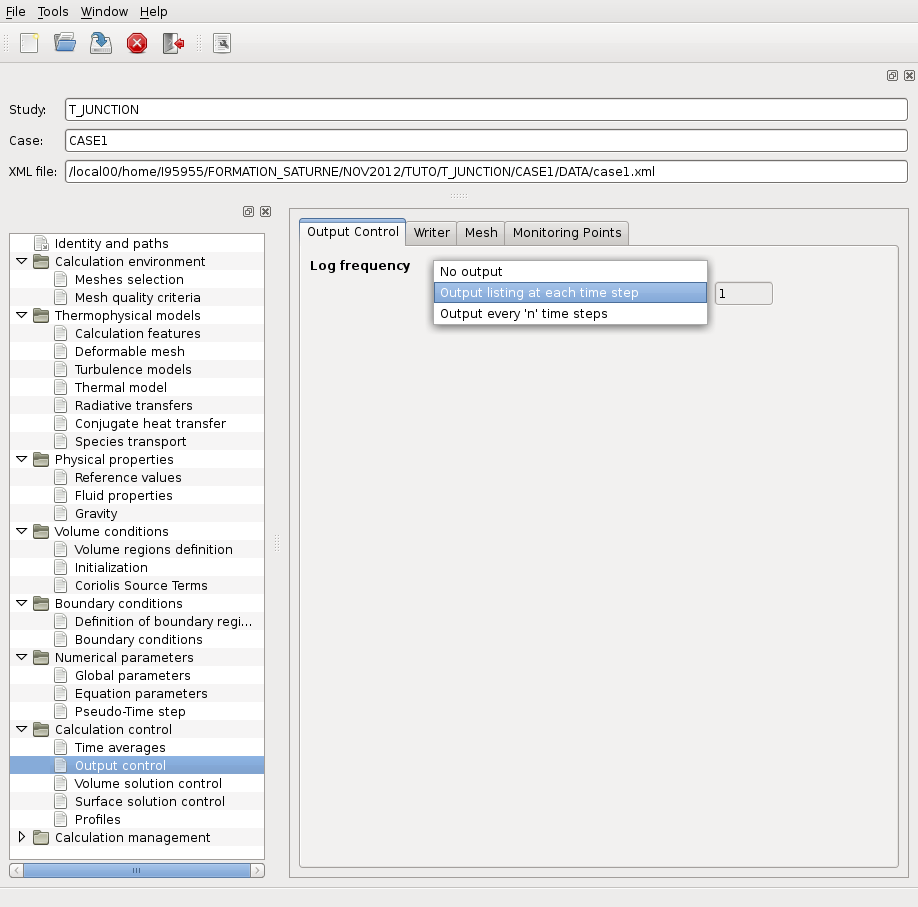
\includegraphics[width=12cm]{case1_V-30}
\caption{Output control: output listing}
\label{fig33_e1}
\end{center}
\end{figure}


\clearpage
For the post-processing (by default \ensight format files), there are three options:\\
\fbox{\begin{minipage}{\textwidth}\texttt{    \\
- Only at the end of calculation\\
- At each time step\\
- Post-processing every 'n' time steps
}\end{minipage} }

In this case, we are interested in the evolution of the variables during the
calculation, so the second option is chosen.

\begin{figure}[ht]
\begin{center}
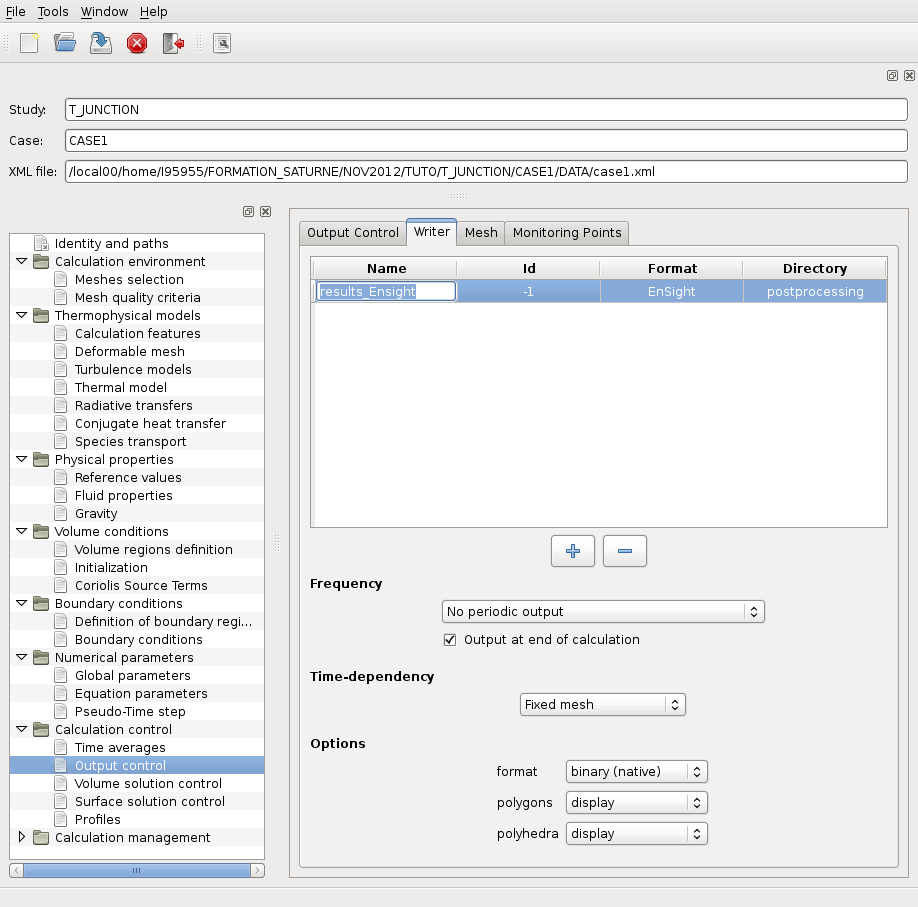
\includegraphics[width=8cm]{case1_V-31}
\caption{Output control: post-processing}
\label{fig34_e1}
\end{center}
\end{figure}


\clearpage
The other options are kept to their default value.

\begin{figure}[ht]
\begin{center}
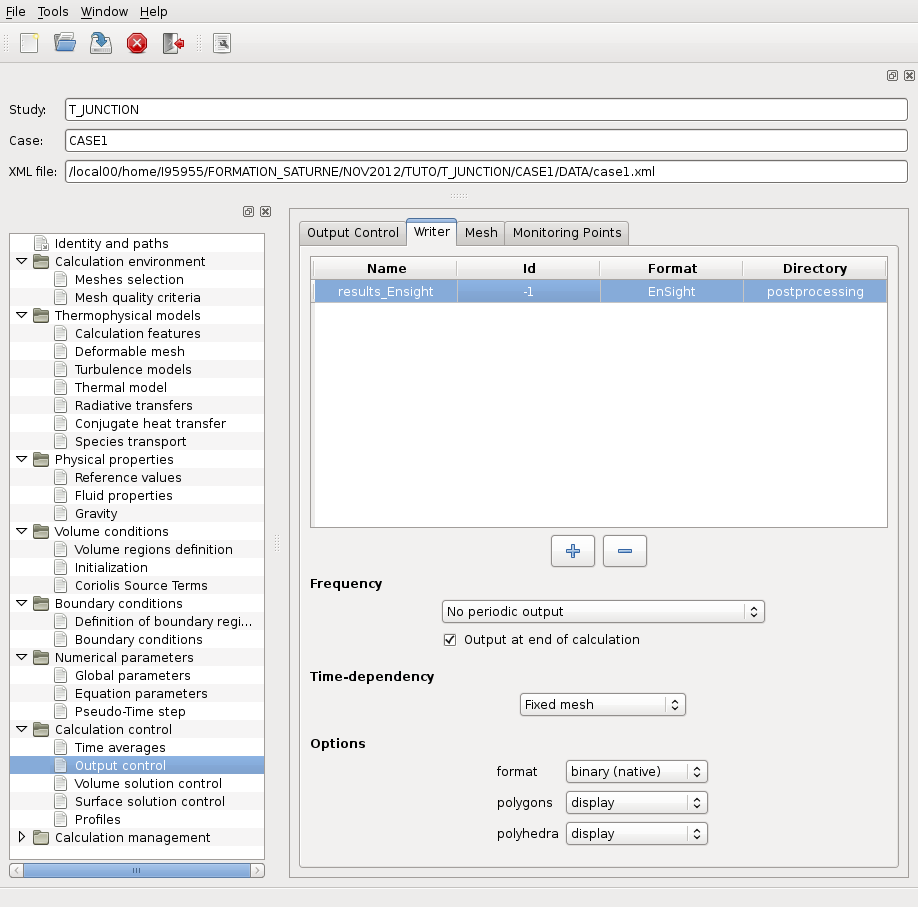
\includegraphics[width=8cm]{case1_V-32}
\caption{Output control}
\label{fig35_e1}
\end{center}
\end{figure}

The {\itshape Monitoring Points} tab allows to define specific points
in the domain (monitoring probes) where the time evolution of the different
variables will be stored in historic files. In this case no monitoring points
are defined.


\clearpage
The {\itshape Volume solution control} item allows to specify which variable will
appear in the output listing, in the post-processing files or on the
monitoring probes. In this case, the default value is kept, where every variable
is activated.


\begin{figure}[ht]
\begin{center}
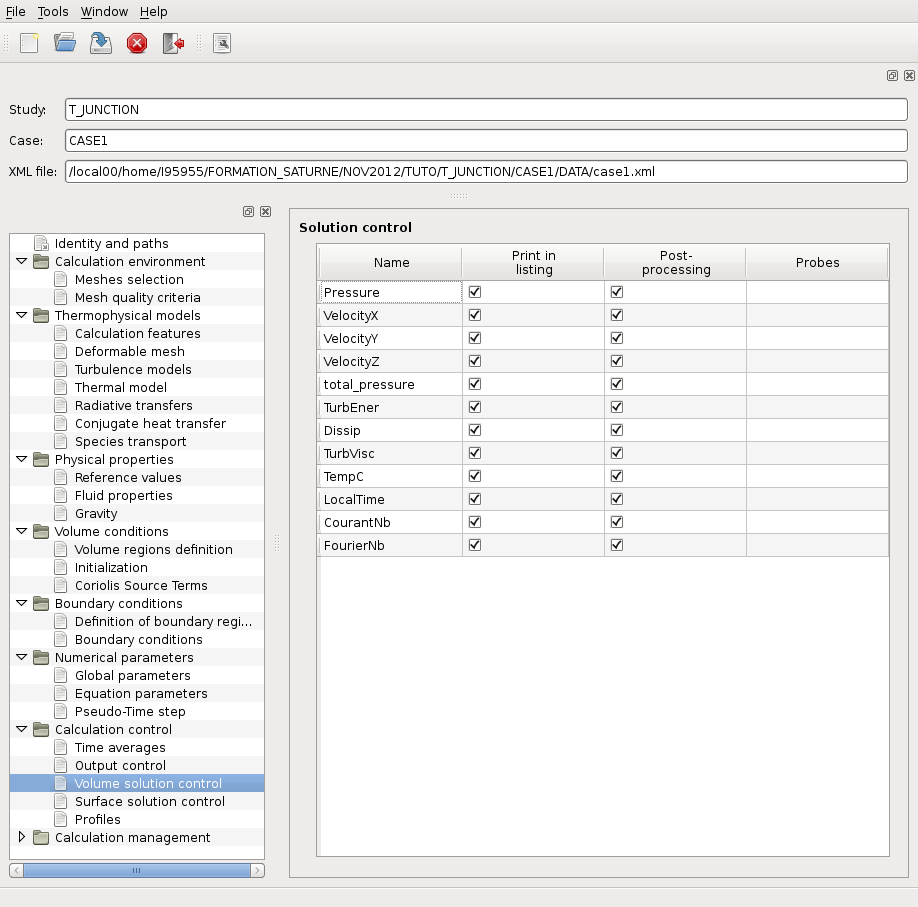
\includegraphics[width=12cm]{case1_V-33}
\caption{Solution control}
\label{fig36_e1}
\end{center}
\end{figure}


\clearpage
The {\itshape Start/Restart} item allows to start a new calculation from the
results of a former one. It is not the case in the present calculation so
nothing has to be modified.

\begin{figure}[ht]
\begin{center}
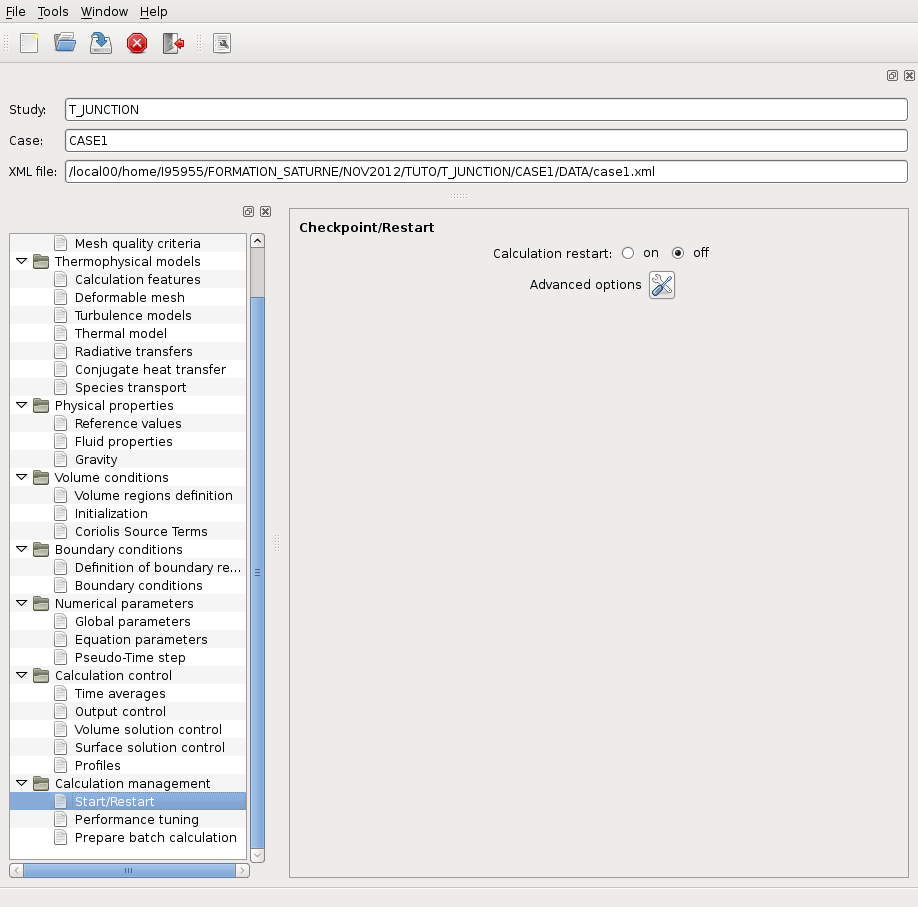
\includegraphics[width=12cm]{case1_V-34}
\caption{Start/Restart}
\label{fig40_e1}
\end{center}
\end{figure}


\clearpage
The final item, {\itshape Prepare batch calculation}, is used to prepare the launch
script and, on certain architectures, launch the calculation.

\begin{figure}[ht]
\begin{center}
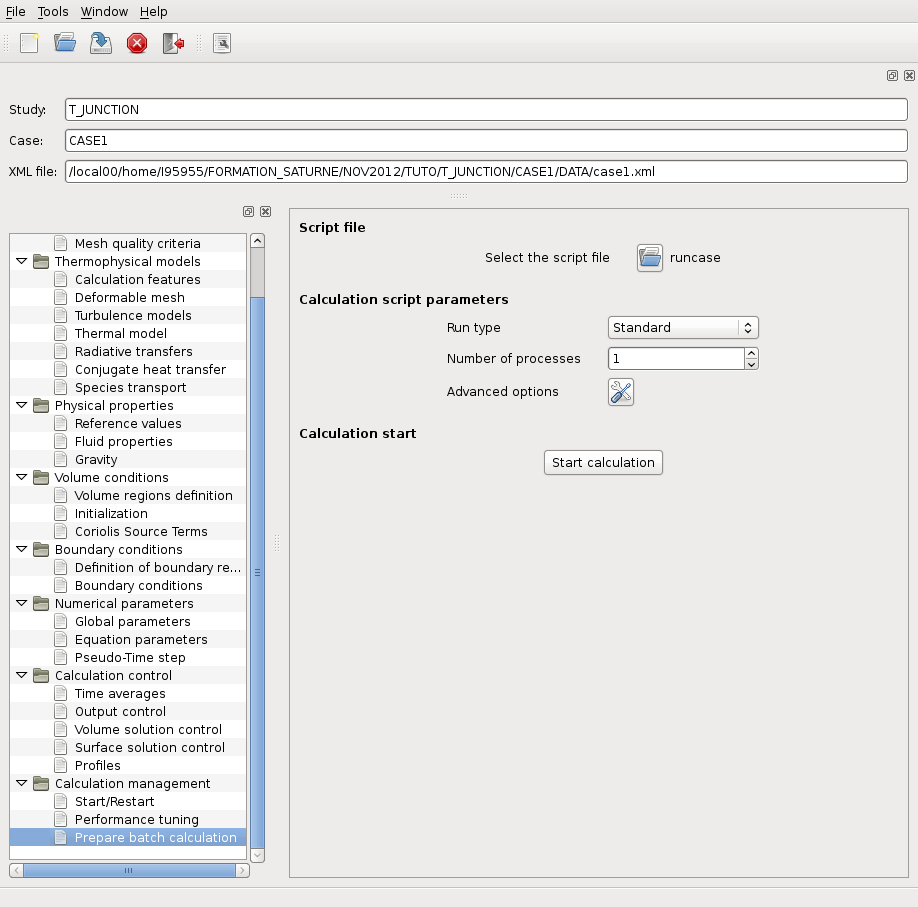
\includegraphics[width=10cm]{case1_V-35}
\caption{Prepare batch analysis: Computer selection}
\label{fig41_e1}
\end{center}
\end{figure}


\clearpage
Click on the icon to {\itshape Select the batch script file} to select the
launch script. The default launch script is named \texttt{runcase} and is
located in the \texttt{SCRIPTS/} directory. Select it and click on {\itshape Open}.

Remember to save the \texttt{xml} file before opening the launch script.

\begin{figure}[ht]
\begin{center}
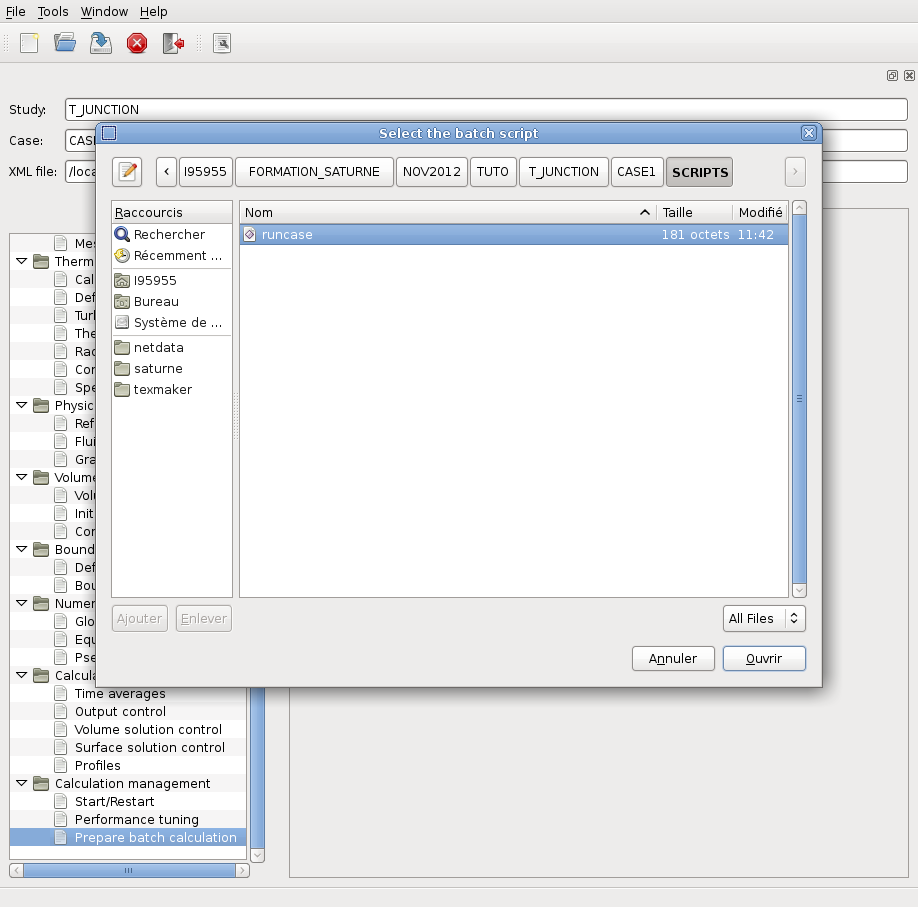
\includegraphics[width=12cm]{case1_V-36}
\caption{Prepare batch analysis: batch script file selection}
\label{fig42_e1}
\end{center}
\end{figure}


\clearpage
When the script is selected, new options will appear.
On this calculation, the number of processors used will be left to 1.

%When launching a calculation, a temporary directory is created on the machine,
%where the script copies and creates temporary files and from where the \CS
%executable is launched. Should some user routines read or write case-specific
%files, they must be copied in the temporary directory, or from the temporary
%directory into the RESU directory. The {\itshape User files} icon allows the
%user to specify user data files (in the DATA directory) or user result files,
%that will then be copied automatically to or from the temporary directory.
%In this example, no user file is needed.

Finally, the {\itshape Advanced options} icon allows to change some more
advanced parameters that will not be needed in this simple case.

Eventually, save the \texttt{xml} file and execute it by clicking on
 {\itshape start calculation}. The results will be copied in the \texttt{RESU/}
directory.

\begin{figure}[ht]
\begin{center}
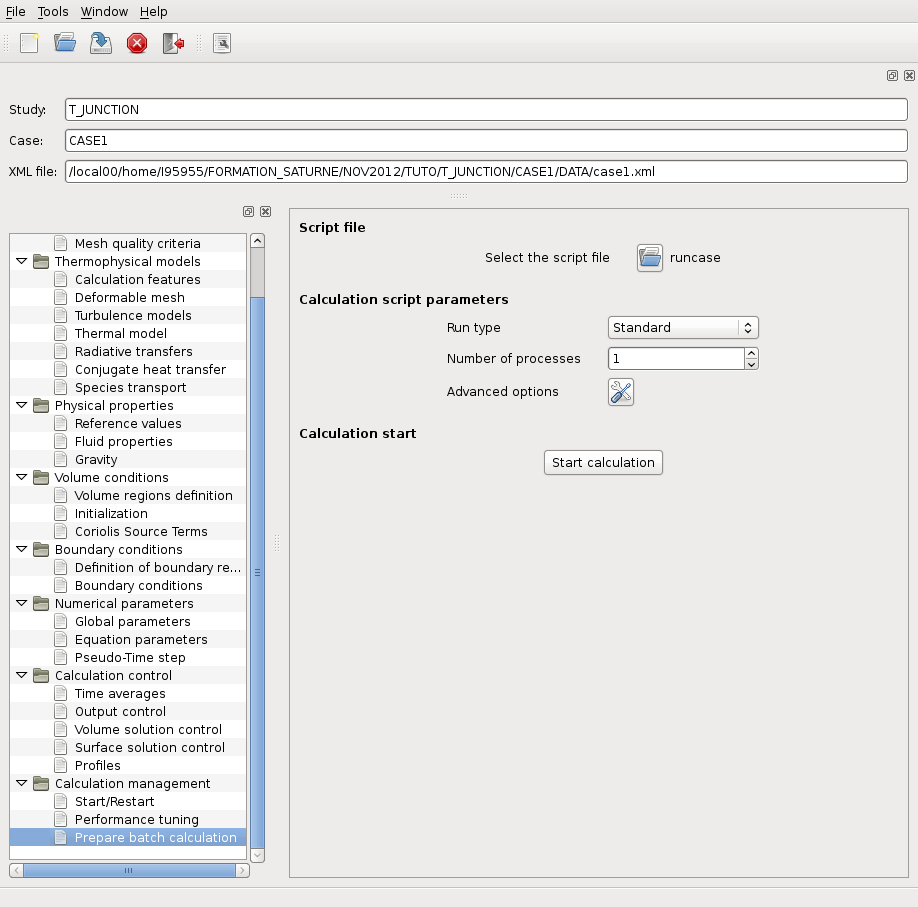
\includegraphics[width=10cm]{case1_V-37}
\caption{Prepare batch analysis: Execution}
\label{fig43_e1}
\end{center}
\end{figure}


\begin{figure}[ht]
\begin{center}
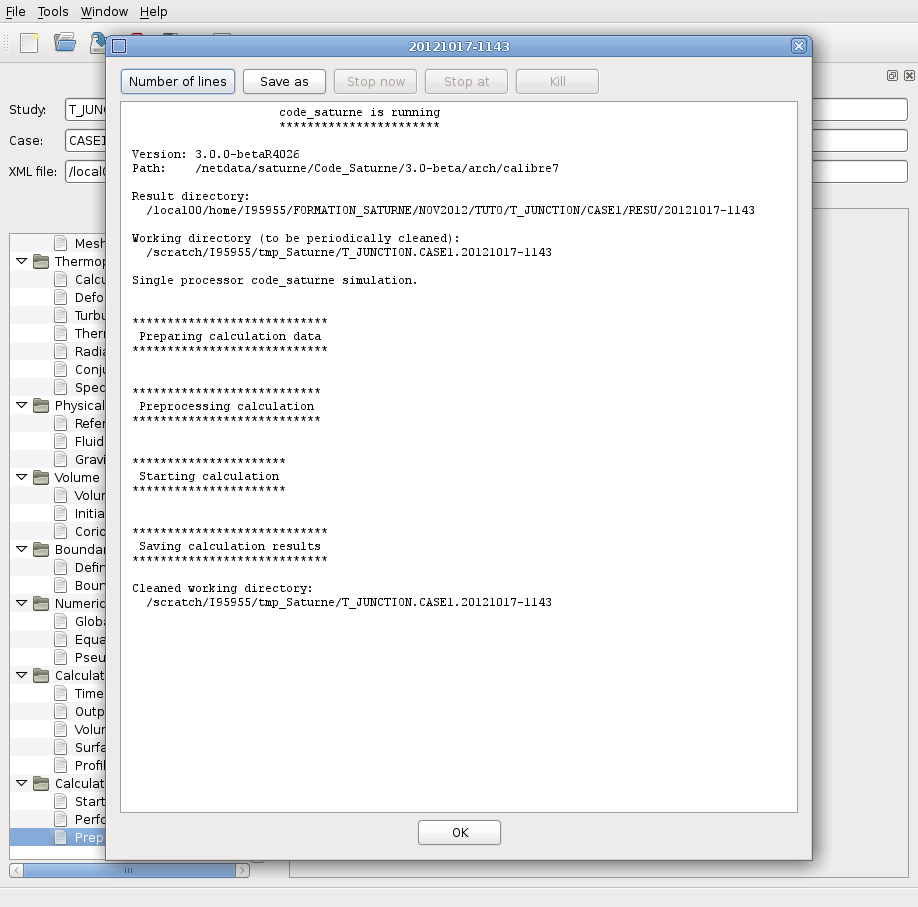
\includegraphics[width=10cm]{case1_V-38}
\caption{Run}
\label{fig43_e1}
\end{center}
\end{figure}
